% \RequirePackage[l2tabu, orthodox]{nag} % Warn about outdated commands/packages.
% The report class uses some outdated commands, about which nag will complain.
% You can just ignore these warnings.

\documentclass[11pt, a4paper]{report} % Sets font and paper size.

%%% General formatting packages (order is important, so don't sort) %%%
\usepackage{amsmath} % More equation formatting.
\usepackage[dutch, english]{babel} % Language specific quirks.
\usepackage{booktabs} % Improved tables.
\usepackage[font=small]{caption} % Better caption formatting.
\usepackage{fancyhdr} % Modification of headers and footers.
\usepackage[T1]{fontenc} % Makes one unicode character of special input (e.g. ö).
\usepackage[margin=1.25in]{geometry} % Control page layout.
\usepackage{float} % More control over image positions.
\usepackage{graphicx} % Include graphics. Use '\graphicspath' to locate files in a different folder.
\usepackage[utf8]{inputenc} % Special characters (e.g. trema) can be entered directly: .tex file has to be saved using UTF-8 encoding.
\usepackage{lmodern} % Alternative font because 'fontenc' package does not work with default.
\usepackage{microtype} % Improves character spacing.
\usepackage[sort]{natbib} % Provides (author, year) references. \citet: textual, \citep: parenthetical
\usepackage{physics} % Provides physics macros such as Dirac notation.
\usepackage{tikz} % Draw diagrams and figures.
\usepackage{url} % Allow inclusion of urls in text.
\usepackage{siunitx} % SI unit formatting and scientific notation.
\usepackage{subcaption} % Allow subcaptions.
\usepackage[nottoc]{tocbibind} % Include references in table of contents.
\usepackage[colorinlistoftodos]{todonotes} % Add todo notes.
\usepackage{cleveref} % Automate "equation (...)" reference. Use \vref.
\usepackage{commath}
\usepackage{breqn}
\usepackage{adjustbox}

%%% Additional options %%%
\pagestyle{fancy} % Set header style.
\setlength{\headheight}{14pt}
\fancyhead[R]{\rightmark}
\fancyhead[L]{}


%%% Personal Information %%%
\newcommand\TITLE{Monte Carlo Simulations of the 3-State Potts Model in 2D}
\newcommand\THESISFORM{Bachelor Project Physics and Astronomy, 15 EC\\conducted between 29-03-2016 and xx-xx-2016\\submitted on xx-xx-2016}
\newcommand\INSTITUTE{Instituut voor Theoretische Fysica Amsterdam}
\newcommand\FACULTY{Faculteit der Natuurwetenschappen, Wiskunde en Informatica}
\newcommand\UNIVERSITY{Universiteit van Amsterdam}
\newcommand\AUTHOR{Teun Zwart (10499873)}
\newcommand\SUPERVISOR{dr. Phillipe Corboz}
\newcommand\SECONDASSESSOR{dr. Edan Lerner}
\newcommand\UNIVERSITYLOGO{UvA-logo.png} % Uncomment line below and add name of logo file.

\graphicspath{{./images/}}


\begin{document}

\begin{titlepage}
	\begin{center}
		\rule{\textwidth}{0.4mm}\\[0.5cm]
		\huge{\textbf{\TITLE}}
		\rule{\textwidth}{0.4mm}\\[0.5cm]\todo{Dates to be filled.}
		\large{\THESISFORM}\\[0.5cm]
		\begin{minipage}[t]{0.4\textwidth}
			\begin{flushleft}
				\large\emph{Author}\\{\AUTHOR}
			\end{flushleft}
		\end{minipage}
		\begin{minipage}[t]{0.4\textwidth}
			\begin{flushright}
				\large\emph{Supervisor}\\{\SUPERVISOR}\\~\\
				\large\emph{Second Assessor}\\{\SECONDASSESSOR}
			\end{flushright}
		\end{minipage}
		\vfill
		\large{\INSTITUTE}\\
		\large{\FACULTY}\\
		\large{\UNIVERSITY}\\~\\
		\includegraphics[width=1.5cm]{\UNIVERSITYLOGO}
	\end{center}
\end{titlepage}

\thispagestyle{plain}
\section*{Abstract}

We studied the critical behaviour of the 3-state Potts model in two dimensions and zero-field.
Monte Carlo simulations were used to find the critical temperature, as well as the critical exponents of the model.
These values were calculated by using finite size scaling methods.
The Ising model in two dimensions was used as a benchmark for the methods used, given that it is exactly solved.
The values found for the critical exponents as well as the critical temperature for the Potts model were in agreement with the values found in the literature which were determined using Monte Carlo simulations, as well as conjectured exact values.


\newpage
\thispagestyle{plain}
\section*{Populaire Samenvatting}
Faseovergangen zien we overal om ons heen. Water verandert in stoom, of bevriest tot ijs.
Bij een faseovergang zien we dat een bepaald getal, dat we de orde parameter noemen, een sprong maakt.
Bij een magneet is dat bijvoorbeeld de magnetisatie, die een waarde heeft bij lage temperaturen maar 0 wordt als de magneet wordt opgewarmd tot boven zijn Curie temperatuur.

In dit verslag beschrijf ik de faseovergang van twee modellen.
Het Ising model beschrijft een rooster waarbij op ieder roosterpunt een klein magneetje zit (dat we een spin noemen), die omhoog of omlaag kan wijzen.
Het Potts model veralgemeniseerd dit idee door iedere spin in een richting te laten wijzen die gelijk verdeelt zijn over een cirkel.

De faseovergangen worden onderzocht met behulp van Monte Carlo computer simulaties.
Deze simulaties zijn bijvoorbeeld ook nuttig bij het

\todo{• Covers 300-600 words with at least one picture, but altogether fits on one A4,
• Is by itself understandable at secondary school level,
• Explains the key message of the research in an enthusiastic and attractive way,
• Invites to read the rest of the report.}

\tableofcontents

\chapter*{Introduction}
\addcontentsline{toc}{chapter}{Introduction}
\todo{Motivation for the research conducted.
• Introduction to the theoretical background.
• Scientific questions.
• Approach.}
Phase transitions are an everyday part of life, the most well known being the transition of water into water vapour or ice into water.
They also occur in more abstract contexts such as networks of neurons.\cite{tkacik:2015}

Although there are some systems that can be exactly solved and thus be studied at the phase transition, many more cannot, and thus different methods have to be employed to understand the phase transitions.
In this thesis we will use Monte Carlo simulations to study the critical behaviour of the Potts model.
We proceed as follows:

In Chapter 1 we consider exactly what properties a phase transitions has.
We see that the behaviour of many thermodynamic properties of a system at criticality can be described by critical exponents.
These exponents are closely related to each other.
We also consider the two-dimensional Ising model in zero-field, which has been solved exactly and for which the critical exponents are known.
Then we have a look at the Potts model, its definition and some conjectures concerning properties of the phase transition.

In Chapter 2 we look at the theory behind simulating lattice systems using Monte Carlo simulations.
We define the Metropolis algorithm, what shortcomings it has and how those shortcomings can be amended by using the Wolff algorithm.
We also consider some optimisations for the simulations.

Chapter 3 lays out the way to analyse the data obtained from the simulation.
Some care has to be taken to use statistically independent measurements.
We also look at resampling methods used to calculate properties of the system that depend in a complicated way on the measured quantities.
The critical temperature is found by using Binder cumulants, while critical exponents are found using finite size scaling arguments.

In Chapter 4 the results of applying the methods from Chapter 3 are presented for the two-dimensional Ising and Potts models.
The measured values for the critical temperatures and exponents agree well with the exact solution (for the Ising model) and other simulation and conjectures (for the Potts model).

In Chapter 5 we summarise the results and give an outlook for further work.

Due to the strong computational component of this project, a significant chunk of code is not included here.
A repository containing Python and Cython\footnote{Cython is a Python module that allows the inclusion of static types and other C features in Python code and converts the resulting code into valid C, which is then normally compiled. Especially for-loop heavy code may become 300 times faster. See \url{cython.org}} code as well as the data sets that were generated may be found at \url{github.com/teunzwart/bachelor-project}, including a basic guide on how to use it.\todo{Currently this repository is still private.}

Finally I would like to thank my supervisor, dr. Phillipe Corboz, for introducing me into the field of computational physics and patiently explaining statistical analysis of Monte Carlo data.
I would also like to thank Edan Lerner for acting as my second assessor.

\chapter{Models and Critical Phenomena}

\section{Phase Transitions and Critical Phenomena}
To determine when a phase transition has taken place, we consider the order parameter.
In ferromagnetic systems such as iron, as well as in the systems we will study in this work, this is the magnetisation.
On one side of the phase transition a non-zero magnetisation is present.
As the iron is heated, it moves past its Curie temperature and the magnetisation does become zero.
More generally we consider an order parameter \(\phi\) which is a quantity that is non-zero on one side of the phase transition, and vanished on the other side. Usually the order parameter is zero on the high temperature side of the phase transition. (See \cref{fig:ising_magnetization}. The Ising model is considered in more detail in \cref{sec:ising_model}.)
The temperature at which the order parameter becomes zero is the critical temperature \(T_c\).
\begin{figure}[htb]
	\centering
	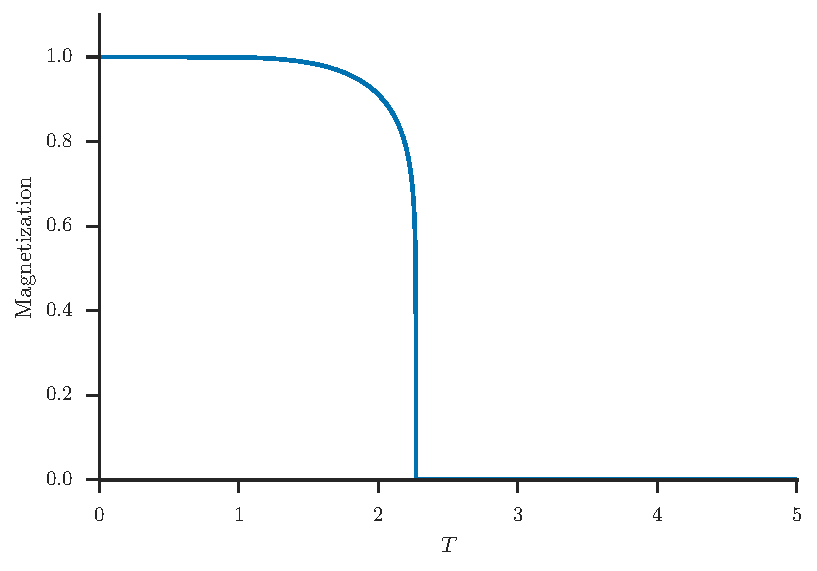
\includegraphics[width=0.66\textwidth]{ising_magnetization}
	\caption{The magnetisation of the two-dimensional Ising model. Notice how the magnetisation is finite on one side of the phase transition, but zero on the other side.}
	\label{fig:ising_magnetization}
\end{figure}

When we consider phase transitions, we distinguish two different kinds.
The phase transition associated with freezing water is what is called first-order.
As the critical temperature is crossed the water molecules move from a disordered phase into an ordered crystal phase.
As this happens, energy is emitted in the form of latent heat.
This is defined as
\begin{equation}
	\label{eq:latent_heat}
	l = \int_{T_c-}^{T_c+} c(T) \dif T,
\end{equation}
with \(l\) the latent heat and \(c(T)\) the heat capacity of the system.
In first order transition the order parameter is discontinuous at \(T_c\).\cite{binney:1992}
In the rest of this work we only consider second-order transitions, for which the latent heat is zero and the order parameter, but not the rate of change of the order parameter is continuous at \(T_c\).

While the latent heat of a transition may be zero, this need not be the case for the heat capacity of the system or other thermodynamic properties such as the magnetic susceptibility.
Often the heat capacity diverges as \(c \propto \abs{T-T_c}^{-\alpha}\).
We call \(\alpha\) a critical exponent.
Because for continuous phase transitions the latent heat has to vanish by definition, \(\alpha\) has to be smaller than 1, because otherwise the integral of \cref{eq:latent_heat} diverges.
No divergence occurs if \(\alpha < 0\).
In the limiting case that \(\alpha = 0\), we can consider the divergence of the specific heat to be logarithmic since
\begin{equation}
	\log(\frac{1}{x}) = \lim_{\alpha \to 0+} \frac{1}{\alpha}\left(x^{-\alpha} - 1\right),
\end{equation}
where \(x = \abs{T - T_c}/T_c\).
Theoretically and experimentally we find that the exponent governing divergence is the same both above and below \(T_c\).\cite{binney:1992}

\subsection{Correlation Functions}
For the systems we would like to consider it is often interesting to quantify how different parts of system relate to each other.
In fact we will see that this correlation proves critical when choosing an appropriate algorithm to numerically study systems around the critical temperature (\cref{sec:critical_slowing_down}).
To quantify the correlations in a system we define the two-point correlation function\cite{binney:1992}, which, to illustrate some properties of the correlation function, we first define for a system of spins:
\begin{equation}
	G^{(2)}(\mathbf{i}, \mathbf{j}) = \langle{\mathbf{s}_i \cdot \mathbf{s}_j}\rangle.
\end{equation}
Here \(\mathbf{i}\) and \(\mathbf{j}\) are the position vectors of the spins at locations \(i\) and \(j\) respectively.
The angle brackets denote thermal averaging.
Because the system is often translationally invariant as well as isotropic, meaning it has no preferred direction, such as in a crystal lattice or in disordered systems, \(G^{(2)}\) often depends only on \(\abs{\mathbf{i} - \mathbf{j}} \)

In the general case the two-point correlation function is defined as
\begin{equation}
	G^{(2)}(r) = \langle \boldsymbol{\phi}(0) \cdot \boldsymbol{\phi}(\mathbf{r}) \rangle,
\end{equation}
where \(\phi\) is the order parameter of the system.
Below \(T_c\) the system is ordered and \(G^{(2)}\) is large for all \(r\).
In the example using spins given above, this means almost all spins are aligned.
A more useful quantity in this case is the connected correlation function
\begin{equation}
	G_c^{(2)} = \langle \boldsymbol{\phi}(0) \cdot \boldsymbol{\phi}(\mathbf{r}) \rangle - \abs{\langle \phi \rangle}^2.
\end{equation}
By subtracting the thermally averaged value of the order parameter from the two-point correlation function, we can ignore the general alignment of the order parameter and only have fluctuations in the order parameter contribute.

When \(T/T_c\) is either large or small \(G_c^{(2)}\) is small.
Precisely at the critical temperature \(G_c^{(2)}\) has the form
\begin{equation}
	G_c^{(2)} \propto \frac{1}{r^{d-2+\eta}},
\end{equation}
with \(d\) the dimensionality of the system and \(\eta\) another critical exponent.
Far away from \(T_c\) \(G_c^{(2)}\) can not be approximated by a power law, but for \(\abs{T-T_c} / T_c \ll 1\) \(G_c^{(2)}\) has the form
\begin{equation}
	G_c^{(2)} \propto \frac{e^{-r/\xi}}{r^{d-2+\eta}}.
\end{equation}
\(\xi\) denotes the correlation length.
Fluctuations of the order parameter up to this length scale are common, but larger fluctuations are exponentially suppressed.
The correlation length diverges as \(T_c\) is approached from above or below, according to
\begin{equation}
	\label{eq:correlation_length}
	\xi \propto \abs{T-T_c}^{-\nu},
\end{equation}
where \(\nu\) is another critical exponent.

\subsection{Scaling Laws}\label{sec:scaling_laws}
We can define three other critical exponents.
For the magnetic susceptibility we have
\begin{equation}
	\label{eq:chi_divergence}
	\chi \propto \abs{T-T_c}^{-\gamma},
\end{equation}
while for the magnetisation of a system we have
\begin{equation}
	\label{eq:magnetization_beta}
	m \propto \abs{T-T_c}^{\beta} \mathrm{\ \ \ \ \ T \to T_c\ from\ below}.
\end{equation}
Finally we can define a critical exponent for the magnetisation in a non-zero magnetic field (the previous five critical exponents assumed \(B=0\)).
Precisely at \(T_c\)
\begin{equation}
	m \propto B^{1/\delta} \mathrm{\ \ \ \ \ B \to 0}.
\end{equation}

These six critical exponents are not independent of each other but are related through scaling laws.
Given these scaling laws only two critical exponents need to be known to determine all others as well.
They are:
\begin{align}
	\alpha + 2\beta +\gamma &= 2\\
	\alpha + \beta(\delta+1) &= 2\\
	(2-\eta)\nu &= \gamma \\
	\nu d &= 2- \alpha,
\end{align}
with \(d\) the dimensionality of the system.\cite{binney:1992,baxter:1989,landau:2015}


\subsection{Universality}
One property of critical phenomena that simplifies their study is the concept of universality.
This is the independence of many thermodynamic properties on the exact details of the hamiltonian of the system.
They will only depend on the dimensionality of the system and symmetries of the Hamiltonian
Consider the hamiltonian
\begin{equation}
	H(s) = H_0(s) + \lambda H_1(s),
\end{equation}
where \(s\) denotes the state of the system, \(H_0\) is a part with a given symmetry, and \(H_1\) does not have that symmetry.
The critical exponents then only depend on \(\lambda\) in that they have one value when \(\lambda=0\) and another when \(\lambda \neq 0\).
This also means that, if both \(H_0\) and \(H_1\) have the same symmetries, then, if \(H_0\) is some simple hamiltonian while \(H_1\) is more complicated, it is possible to obtain the critical exponents of a system using the simple part while stripping the more complicated part.
This may significantly ease the determination of critical exponents when performing simulations.
Different systems with the same critical exponents are said to be in the same universality class.
It is believed (and experimentally established with error) that such diverse systems as carbon dioxide, xenon and the three-dimensional Ising model are in the same universality class.\cite{baxter:1989}

\section{The Two-Dimensional Ising Model}\label{sec:ising_model}

To validate methods to determine critical exponents for systems that are not exactly solvable, a control system that is exactly solved is useful. To that end we study the two-dimensional Ising model in zero-field, first solved exactly in 1944 by Lars Onsager.\cite{onsager:1944}
It describes a square lattice with nearest neighbour interactions, where each lattice point has with it associated a number (which we will refer to as spin) which may either be +1 or -1 and was originally meant as a model for magnets.
The Hamiltonian in zero-field is\cite{mccoy:1973}
\begin{align}
	H = -J_{1} \sum_{j=1}^{\mathcal{M}} \sum_{k=1}^{\mathcal{N}} \sigma_{j,k} \sigma_{j,k+1} - J_{2} \sum_{j=1}^{\mathcal{M}} \sum_{k=1}^{\mathcal{N}} \sigma_{j,k} \sigma_{j+1,k},
\end{align}
with \(\mathcal{M}\) and \(\mathcal{N}\) the extent of the lattice in the \(x\)- and \(y\)-directions respectively and \(J_{1}\) and \(J_{2}\) the interaction strength between neighbours in respectively the \(x\)- and \(y\)-directions.
In the case where the interaction strength in both directions is the same the Hamiltonian becomes\cite{newman:1999}
\begin{align}
	\label{eq:isotropic_hamiltonian}
	H = -J \sum_{\langle ij \rangle} \sigma_{i} \sigma_{j},
\end{align}
where the bracket denotes summation over nearest neighbours.\footnote{Note that naively applying this Hamiltonian to calculate the lattice energy overcounts the energy by a factor of 2 since each bond is counted twice.}
In the ferromagnetic ground state (\(J>0\)) all spins on the lattice are aligned in one of two possible directions (the direction is chosen when the mirror symmetry in the lattice plane is spontaneously broken as the lattice cools).
The Hamiltonian is subject to toroidal boundary conditions in both directions, meaning \(\sigma_{1,k} = \sigma_{\mathcal{M}+1,k}\) and \(\sigma_{j,1} = \sigma_{j,\mathcal{N}+1}\).
We are interested in the thermodynamic properties of the Ising Model.
To that end we define the partition function
\begin{align}
	Z &= \sum_{\sigma = \pm 1} e^{-\beta H} \\
	  &= \sum_{\sigma = \pm 1} \prod_{j=1}^{\mathcal{M}} \prod_{k=1}^{\mathcal{N}} e^{\beta J_1 \sigma_{j,k} \sigma_{j,k+1}} \prod_{j=1}^{\mathcal{M}} \prod_{k=1}^{\mathcal{N}} e^{\beta J_2 \sigma_{j,k} \sigma_{j+1,k}},
\end{align}
with \(\beta=1/k_B T\) and the sum running over every possible orientation of the spins on the lattice. Solving this requires a non-trivial amount of effort and it is best to refer to either Onsager\cite{onsager:1944}, who systemically added one-dimensional Ising models together to create a two dimensional lattice, or Kasteleyn as described in \cite{mccoy:1973}, whose approach considerably simplifies the derivation by reducing it to a combinatorial problem.

The derivation introduces a sign ambiguity in \(Z\) which takes some additional care to resolve, but we can avoid having to deal with this by considering the free energy \(F\) in the thermodynamic limit\footnote{This is the limit in which the number of particles on the lattice tends to infinity.} instead of the partition function
\begin{dgroup*}
	\begin{dmath*}
		F = -\frac{1}{\beta} \lim_{\substack{\mathcal{N} \to \infty \\ \mathcal{M} \to \infty}} \frac{1}{\mathcal{M} \mathcal{N}} \log({Z_{\mathcal{M}, \mathcal{N}}})
	\end{dmath*}
	\begin{dmath}
		= -\frac{1}{\beta} \left[ \log(2) + \frac{1}{2} \frac{1}{(2\pi)^2} \int_{0}^{2\pi} \dif \theta_{1} \int_{0}^{2\pi} \dif \theta_2 \log \bigg(\cosh{(2\beta J_1)} \cosh{(2\beta J_2)} - \sinh{(2\beta J_1)} \cos{(\theta_1)} - \sinh{(2\beta J_2)} \cos{(\theta_2)}\bigg) \right].
	\end{dmath}
\end{dgroup*}

\(F\) is an analytic function of the temperature \(T\), except at one value, which we will call the critical temperature \(T_c\). At this temperature we can define the equality\cite{mccoy:1973}
\begin{align}
	\abs{z_1} &= \frac{1 - \abs{z_2}}{1+ \abs{z_2}}, \text{ with } z_1 = \tanh(2\beta J_1), z_2 = \tanh(2\beta J_2).
\end{align}
Rewriting and squaring this gives
\begin{align}
	\label{eq:ising_z_functions}
	1 - \abs{z_1 z_2} &= \abs{z_1} + \abs{z_2}\rightarrow\\
	\left(1 - z_1^2 \right) \left(1 - z_2^2 \right) &= 4 \abs{z_1 z_2}
\end{align}
Finally, using
\begin{align}
	\frac{1}{2 z_k}\left(1 - z_k^2\right) = \frac{1}{\sinh(2 \beta J_k)}, \text{ with } k \in \{{1, 2}\}
\end{align}
we get the equality
\begin{align}
	1 = \sinh(2\beta J_1) \sinh(2\beta J_2).
\end{align}
In the case where interaction strength in both the \(x\)- and \(y\)-directions is the same (\(\abs{J_1} = \abs{J_2} = J\)) we get an expression for the critical temperature in terms of the bond energy
\begin{align}
	1 &= \sinh(2\beta J) \to \\
	k_B T_c &= \frac{2}{\text{asinh}(1)}J = \frac{2}{\log(1+\sqrt{2})}J \approx 2.269 J
\end{align}
Onsager \cite{onsager:1944} also calculated the values of the free energy, internal energy and entropy at the critical temperature\footnote{We use lowercase letters to denote the thermodynamic properties of a single spin on the lattice and uppercase letters when referring to the entire lattice. Taking as an example the internal energy, \(U/N = u\) with \(N\) the number of spins on the lattice.}:
\begin{align}
	-\frac{f_c}{k_B T} &= \frac{1}{2} \log{2} + \frac{2}{\pi} G \approx 0.929, \\
	u_c &= - \sqrt{2} J \approx - 1.414 J,\\
	\frac{s_c}{k_B} &= \log{(\sqrt{2} e^{2G/\pi})} - \sqrt{2} \frac{J}{k_B T} \approx 0.306
\end{align}
with \(G\) Catalan's constant.\footnote{\(G = 1^{-2} - 3^{-2} + 5^{-2} - 7^{-2} +\ldots \approx 0.916\)}

\subsection{Thermodynamic Properties of the Two-Dimensional Ising Model}
From the free energy it is relatively simple to determine the specific heat per spin and the internal energy per spin by taking the appropriate derivatives of the free energy\cite{mccoy:1973}. We work with the isotropic case where \(\abs{J_1} = \abs{J_2} = J\) and \(z_1 = z_2 = z = \tanh(\beta J)\), corresponding to \cref{eq:isotropic_hamiltonian}.
Then the expression for the free energy becomes
\begin{dmath}
	F = -\frac{1}{\beta} \left[\log(2\cosh^2(\beta J)) + \log(1+z^2) + \frac{1}{2\pi^2} \int_0^{\pi}\dif \theta_1 \int_0^{\pi} \dif \theta_2 \log(1-\frac{1}{2}k \Big\{\cos(\theta_1) + \cos(\theta_2)\Big\})\right],
\end{dmath}
with
\begin{align}
	\label{eq:elliptic_argument}
	k = \frac{4z(1-z^2)}{(1+z^2)^2} = \frac{2\sinh(2\beta J)}{\cosh^2{(2\beta J)}}.
\end{align}
Performing the substitutions \(\omega_1 = \frac{1}{2}(\theta_1 + \theta_2)\) and \(\omega_2 = \frac{1}{2}(\theta_1 - \theta_2)\) and integrating over \(\omega_1\) the free energy becomes
\begin{align}
		F &= -\frac{1}{\beta} \left[\log(2\cosh(2\beta J)) + \frac{1}{\pi^2} \int_0^{\frac{\pi}{2}} \dif \omega_1 \int_0^{\frac{\pi}{2}} \dif \omega_2 \log(1- k \cos(\omega_1)\cos(\omega_2))\right]\\
		&= -\frac{1}{\beta} \left[\log(\sqrt{2}\cosh(2\beta J)) + \frac{1}{\pi} \int_0^{\frac{\pi}{2}} \dif \omega \log(1+\left\{1-k^2 \cos^2(\omega)\right\}^{\frac{1}{2}}) \right]
\end{align}

We will take derivatives from this expression to determine expressions for thermodynamic properties. The internal energy per spin is
\begin{align}
	\label{eq:internal_energy}
	u &= \frac{\partial \beta F}{\partial \beta}\\
	&= -2 J \tanh(2\beta J) + k \frac{\dif k}{\dif \beta} \frac{1}{\pi} \int_0^{\frac{\pi}{2}} \dif \omega \frac{\sin^2(\omega)}{\Delta (1+\Delta)}
\end{align}
with
\begin{align}
	\Delta = \left( 1 - k^2 \sin^2(\omega) \right)^{\frac{1}{2}}.
\end{align}

Note that the argument of the integral in \cref{eq:internal_energy} can be rewritten as
\begin{align}
	\frac{\sin^2(\omega)}{\Delta (1+\Delta)} = \frac{(1 - \Delta) \sin^2(\omega)}{\Delta(1-\Delta^2)} = \frac{1}{k^2}\left(\frac{1}{\Delta} - 1\right),
\end{align}
from which it follows that
\begin{align}
	u = - 2 J \tanh(2\beta J) + \frac{1}{\pi} \frac{1}{k} \frac{\dif k}{\dif \beta} \left[ K(k) - \frac{\pi}{2}\right].
\end{align}
Here \(K(k)\) is the complete elliptic integral of the first kind
\begin{align}
	K(k) = \int_0^{\frac{\pi}{2}} \frac{\dif \phi}{\left(1-k^2 \sin^2(\phi)\right)^{\frac{1}{2}}}.
\end{align}
Taking the derivative of \(k\)
\begin{align}
	\label{eq:k_derivative}
	\frac{1}{k}\frac{\dif k}{\dif \beta} = \frac{2 J}{\tanh(2\beta J)} (1 - 2\tanh^2(2 \beta J)),
\end{align}
the internal energy per spin becomes (see \cref{fig:ising_internal_energy} for a plot)
\begin{align}
	\label{eq:ising_internal_energy}
	u = \frac{-J}{\tanh(2\beta J)} \left[1 + \frac{2}{\pi} \left\{2 \tanh^2(2\beta J) -1 \right\} K(k) \right].
\end{align}

For the specific heat per spin we take the derivative of the internal energy per spin with respect to the temperature
\begin{dgroup}
	\begin{dmath}
		c = \frac{\partial u}{\partial T} \hiderel{=} \frac{-1}{k_B T^2}\frac{\partial u}{\partial \beta}
	\end{dmath}
	\begin{dmath}
		= \frac{J}{k_B T^2} \left[\frac{-2J}{\cosh^2(2\beta J)}\left\{ 1 + \frac{2}{\pi} \left(2 \tanh^2(2\beta J) -1 \right) K(k) \right\}\right]
		+ \frac{16}{\pi} \frac{J}{\tanh^2{2\beta J}} K(k) + {\frac{2}{\pi}\frac{\left(2 \tanh^2(2\beta J) -1 \right)}{\tanh(2\beta J)}\\
		 \frac{\dif k}{\dif \beta} \frac{\dif K(k)}{\dif k}}.
	\end{dmath}
\end{dgroup}
For the derivative of the elliptic integral we use the identity\cite{mccoy:1973}
\begin{align}
	\frac{\dif K(k)}{\dif k} = \frac{1}{k k^{'2}} \left[E(k) - k^{'2} K(k) \right],
\end{align}
where \(E(k)\) is the complete elliptic integral of the second kind
\begin{align}
	\label{eq:elliptic_identity}
	E(k) = \int_0^{\frac{\pi}{2}} \dif \phi \left(1-k^2 \sin^2(\phi)\right)^{\frac{1}{2}},
\end{align}
and \(k^{'2} = 1 - k^2\).
Using \cref{eq:k_derivative} and \cref{eq:elliptic_identity} the expression for the specific heat per spin becomes (see \cref{fig:ising_internal_energy} for a plot)
\begin{align}
	\label{eq:ising_heat_capacity}
	c = k_B \left[ \frac{\beta J}{\tanh(2\beta J)} \right]^{2} \frac{2}{\pi} \left[ 2 K(k) -2 E(k) - \left(1 - k' \right) \left\{ \frac{\pi}{2} + k' K(k) \right\}\right].
\end{align}

\begin{figure}[htb]
	\centering
	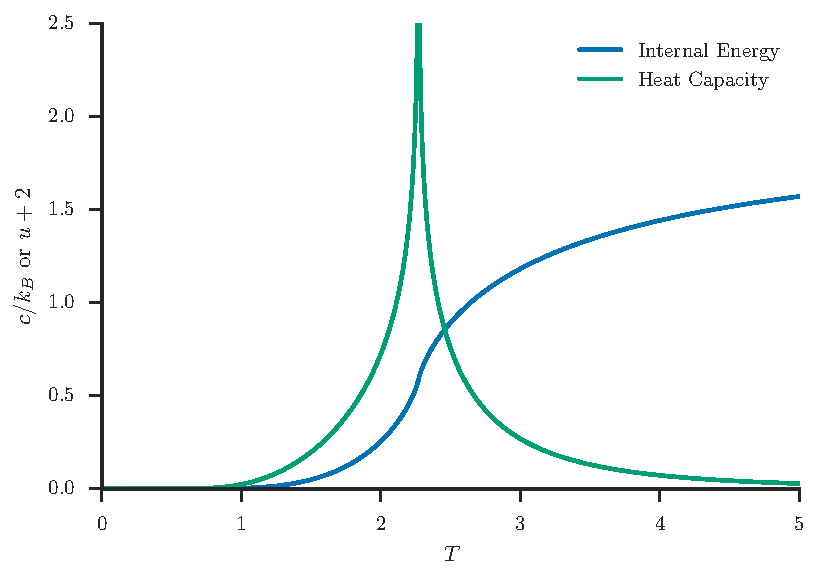
\includegraphics[width=0.66\textwidth]{ising_internal_energy.pdf}
	\caption{The internal energy per site and the specific heat per site of the two-dimensional Ising model in zero-field. Notice the divergence of the specific heat around \(T=T_c \approx 2.269\), which is cutoff in this graph due to the limited resolution.}
	\label{fig:ising_internal_energy}
\end{figure}

\subsection{The Ising Model around \(T_c\)}

Given that we would like to know how the Ising model behaves around \(T_c\), we need to expand the expressions for the internal energy and the heat capacity around this temperature.
When \(T \approx T_c\) the argument \(k\) as defined in \cref{eq:elliptic_argument} of the elliptic integrals in the definitions \cref{eq:ising_internal_energy} and \cref{eq:ising_heat_capacity} becomes approximately 1. More precisely
\begin{align}
	k &\approx 1 - 4 \beta_c^2 J^2 (\frac{T}{T_c} - 1)^2, \\
	k^' &\approx 2 \sqrt{2} \beta_c J (\frac{T}{T_c} - 1)
\end{align}
with \(\beta_c = \frac{1}{k_B T_c}\).
It is obvious that for \(k = 1\) \(E(k) = 1\) whereas \(K(1)\) diverges since the integral becomes
\begin{align}
	\int_0^{\frac{\pi}{2}}\frac{1}{\cos{\theta}} \dif \theta \to \infty
\end{align}
Nevertheless an approximation around \(k = 1\) yields \(K(k) \approx \log(\frac{4}{k^'})\).

At \(T_c\) the internal energy per spin \(u\) does not diverge and has the value
\begin{align}
	u(T_c) = \frac{-J}{\tanh(2\beta_c J)} = -\sqrt{2}J.
\end{align}
The heat capacity per spin \(c\) does diverge. Using the previous expansions
\begin{align}
	\frac{c(T)}{k_B} &\approx \frac{8}{\pi} \left(\beta_c J\right)^2 \left[\log(\frac{4}{k^'})\right] \\
	&= \frac{2}{\pi} \log(1 + \sqrt{2})^2 \left[-\log\abs{\frac{T}{T_c} - 1} - 1 - \frac{\pi}{4} - \log(\frac{\sqrt{2}}{4} \log(1+\sqrt{2}))\right]
\end{align}
and we see \(c\) diverging logarithmically as \(T \to T_c\).
This means that the critical exponents \(\alpha = 0\) for the two-dimensional Ising model.
When Onsager first solved the model, it also highlighted the first instance of universality.
Onsager considered the general case where the interaction energy in the \(x\)- and \(y\)-directions differed, but the logarithmic divergence depended only on the critical temperature, and not on the ratio \(J_1 \ J_2\).\cite{baxter:1989}
Note that the sharp phase transition as described here only occurs when the lattice is of infinite extent.
When we do not operate in the thermodynamic limit the partition function of the Ising model is analytic for all \(T\) and has a maximum but no divergence at \(T_c\).\cite{onsager:1944}


\subsection{Magnetisation of the Ising Model}\label{sec:ising_magnetization}

Onsager also calculated the magnetisation of the Ising model.
On the square lattice with \(T < T_c\) and \(J_1, J_2 > 0\) the magnetisation squared is equal to the spin-spin correlation function
\begin{equation}
	M^2 = \lim_{N \to \infty} \langle \sigma_{00} \sigma_{0,N} \rangle = \lim{N \to \infty} \langle \sigma_{00} \sigma_{N, N} \rangle.
\end{equation}
Determining the correlation function is non-trivial, but the result is
\begin{equation}
	M^2 = \lim_{N \to \infty} \langle \sigma_{00} \sigma_{0,N} \rangle = \left[ \frac{(1-\alpha_1^2)(1-\alpha_2^2)}{(1-\alpha_1 \alpha_2)^2}, \right]^{1/4}
\end{equation}
with
\begin{equation}
	\alpha_1 = \frac{z_1(1-\abs{z_2})}{1+\abs{z_2}}, \alpha_2 = \frac{1}{z_1}\frac{1-\abs{z_2}}{1+\abs{z_2}},
\end{equation}
where we use \(z_1\) and \(z_2\) as defined in \cref{eq:ising_z_functions}.
The magnetisation is then (see \cref{fig:ising_magnetization} for a plot)
\begin{equation}
	M = \left[1 - \left\{\sinh(2\beta J_1)\sinh(2 \beta J_2)\right\}^{-2} \right]^{1/4}.
\end{equation}
When we approach the critical temperature from below we can expand around \(T_c\) and get
\begin{equation}
	M \propto \left[4\beta_c\left\{\frac{J_1}{\tanh(2\beta_c J_1)} + \frac{J_2}{\tanh(2\beta_c J_2)}\right\} \left\{1-\frac{T}{T_c}\right\}\right]^{1/8}.
\end{equation}
Comparing with \cref{eq:magnetization_beta} we see that \(\beta = 1/8\).\cite{wu:1982}

Finally the magnetic susceptibility can be shown to diverge as \(\chi \propto \abs{T - T_c}^{-7/4}\), giving \(\gamma = 7/4\).
With the earlier result \(\alpha=0\), we can use the scaling laws (\cref{sec:scaling_laws}) to determine that \(\delta = 15\), \(\eta = 1/4\) and \(\nu = 1\).\cite{binney:1992}

\section{The Potts Model}
The Potts model was first defined by Potts in 1953 as a generalisation of the Ising model on the suggestion of Domb, his supervisor.\cite{potts:1952}
Domb suggested that that to generalise, we can consider the spins of the model to be confined to a plane, with each spin pointing in one of \(q\) equally spaced directions, separated by an angle \(\theta_n = 2\pi n /q\), with \(n = 0, 1, \ldots q - 1\).
The nearest neighbour interaction depend only on the angle between those neighbours.
The hamiltonian for this system is
\begin{equation}
	H = - \sum_{\langle i, j \rangle} J(\theta_{ij}),
\end{equation}
with \(J(\theta)\) a \(2\pi\)-periodic function and \(\theta_{ij} = \theta_i - \theta_j\) the angle between two spins.
Domb suggested to use \(J(\theta_{ij}) = - \epsilon_1\cos(\theta_{ij})\).
This is now known as the planar Potts model.\cite{wu:1982}

Making use of a duality relation which showed that the partition function at a low temperature \(T\) was equal to that at a high temperature \(T^*\), (\(Z(T)=Z(T^*)\)) Potts found the critical temperature for \(q=2, 3, 4\), by assuming that there is exactly one temperature for which \(T=T^*\).
This method was first used by Kramers and Wannier in 1941\cite{kramers:1941}, to determine the critical temperature of the two-dimensional Ising model three years before Onsager's exact solution.

Potts also gave a formula for the critical temperature of a system with a different interaction strength: \(J(\theta_{ij}) = -\epsilon_2 \delta(\sigma_i, \sigma_j)\), where \(\delta\) is the Kronecker delta.
For this system he established that for all \(q\) the transition occurs at\cite{potts:1952}
\begin{equation}
	\frac{x_0}{x_1} = 1 + \sqrt{q},
\end{equation}
with
\begin{align}
	x_0 &= e^{-J_0 / k_B T} \mathrm{\ \ \ \ \ for\ spins\ in\ like\ orientations,}\\
	x_1 & = e^{-J_1 / k_B T} \mathrm{\ \ \ \ \ for\ spins\ in\ unlike\ orientations}.
\end{align}
For \(q=3\) we find that the critical temperature is \(T_c=\frac{1}{\log(1+\sqrt{3})} \approx 0.995\).\cite{fan:2007}
We call this system the standard Potts model.
Throughout the rest of this thesis we will mainly consider this model and will simply refer to it as the Potts model.
The planar and standard Potts models are related for \(q = 2\) by \(\epsilon_2 = 2 \epsilon_1\) and for \(q=3\) by \(\epsilon_2 = \frac{3}{2} \epsilon_1\).
For the Potts model in two dimensions the transition at the critical point is first-order for \(q > 4\) and second-order for \(q \leq 4\).\cite{wu:1982,baxter:1973}
Potts found that an earlier result by Ashkin and Teller for the discontinuities of the energy and specific heat\cite{ashkin:1943}, \(\Delta E, \Delta C\), could be generalised to show the relationship between those quantities:
\begin{equation}
	\sqrt{q}T \Delta E = \log(\frac{x_0}{x_1}) \Delta E.
\end{equation}
Therefore transitions with a continuos energy exclude the possibility of a discontinuous heat capacity.
This does however not mean that the specific heat needs to be finite at \(T_c\).


At the critical temperature the internal energy is\cite{baxter:1989,binder:1981a}
\begin{equation}
	u_{\mathrm{average}} = -\left(1+\frac{1}{\sqrt{q}}\right)J,
\end{equation}
with
\begin{equation}
	u_{\mathrm{average}} = \frac{1}{2} (u_c^+ + u_c^-),
\end{equation}
where \(u_c^+ = \lim_{T \to T_c^+} \langle u \rangle\) and for a second order transition \(u_c^+ = u_c^-\).
For \(q=3\) (a second order transition) \(u_{\mathrm{average}} = -(1+\frac{1}{\sqrt{3}})J \approx - 1.577 J\).

To properly define when the phase transition occurs we define the order parameter, which here is the magnetisation, as
\begin{equation}
	m = \frac{1}{N}\abs{\sum_i^N e^{i2\pi n_i / q}},
\end{equation}
with the sum running over every site of the lattice, \(N\) being the number of sites and \(n_i\) being the state of the spin at site \(i\).
This is based on the definition of the \(q\)-state Potts model as consisting of equally spaced vectors.
It has the desired properties of being 1 when all spins on the lattice point in the same direction and being 0 when the spins are equally distributed over the possible states.

The Potts model has not been solved exactly, thus we do not know the exact values of the critical exponents.
There are however other systems in the same universality class as the Potts model.
For \(q=2\) the model reduces to the Ising model and associated exponents (\cref{sec:ising_magnetization}).
For \(q=3\) the model is conjectured to be equal to absorbed monolayers (two-dimensional model), a system that can be probed experimentally and gives \(\alpha = 0.36\)\cite{binder:1981a}.
It is also suspected that the hard hexagon model (a two-dimensional lattice model describing a gas of non-overlapping spheres, placed on a triangular lattice so no two molecules are adjacent) is in this universality class.
This model is exactly solved and has the critical exponents\cite{baxter:1989,wu:1982}
\begin{equation}\label{eq:potts_critical_exponents}
	\alpha = \frac{1}{3},\ \ \beta = \frac{1}{9},\ \ \delta = 14,\ \ \nu = \frac{5}{6},\ \ \gamma = \frac{13}{9},\ \ \eta = \frac{4}{15}.
\end{equation}

While no exact solution exists, Den Nijs has put forth conjectures for the values of the exponents.\cite{nijs:1979}
We have\cite{wu:1982}
\begin{equation}
	2 - \alpha = \frac{2}{y_t} ,\ \ \ 1 + \frac{1}{\delta} = \frac{2}{y_h},
\end{equation}
with the thermal and magnetic exponents:
\begin{equation}
	y_t = \frac{3(1-u)}{2-u},\ \ \ y_h = \frac{(3-u)(5-u)}{4(2-u)}.
\end{equation}
For \(q \leq 4\)\cite{wu:1982}
\begin{equation}
	0 \leq u = \frac{2}{\pi} \arccos(\frac{\sqrt{q}}{2}) \leq 1.
\end{equation}
The critical exponents then become\cite{wu:1982, baxter:1989}:
\begin{equation}
	\begin{aligned}[c]
		\alpha &= \frac{2(1-2u)}{3(1-u)}, \\
		\beta &= \frac{1}{12}(1 + u), \\
		\gamma &= \frac{u^2 -4u +7}{6(1+u)}, \\
	\end{aligned}
	\ \ \
	\begin{aligned}[c]
		\delta &= \frac{(3-u)(5-u)}{1-u}, \\
		\nu &= \frac{2-u}{3(1-u)}, \\
		\eta &= \frac{1-u^2}{2(2-u)}.
	\end{aligned}
\end{equation}
For \(q=3\), \(u=1/3\), and these equations reproduce \cref{eq:potts_critical_exponents}.


\chapter{Simulating Lattice Models}

\section{Markov Processes and Monte Carlo Methods}
While some success is to be had by using analytical methods to study lattice models and their critical exponents, often the partition function cannot be determined exactly.
At that point we can use computer simulation of the models in question to study phase transitions, while having exactly solved models as a benchmark for these simulations.

We are almost always interested in the value of a thermal average of a quantity:
\begin{equation}
	\langle X \rangle = \sum_{\alpha}X_{\alpha}p_{\alpha},
\end{equation}
with \(\langle X \rangle\) a thermal average, the sum running over all configurations, each labeled by \(\alpha\), and \(p_{\alpha}\) the Boltzmann probability of state \(\alpha\) in equilibrium\cite{binney:1992}:
\begin{equation}\label{eq:boltzmann_probability}
	p_{\alpha} = \frac{e^{-\beta E_{\alpha}}}{\sum_{\alpha}e^{-\beta E_{\alpha}}}.
\end{equation}
While for small lattices (such as 3 by 3) the number of states is tractable (this number scales as \(2^{N}\) for the Ising model and \(q^{N}\) for the Potts model), for larger lattices the sum can no longer be performed exactly and some clever way has to be found to sample only important states.

Instead, we randomly choose states distributed according to a probability distribution \(p_{\alpha}\).
If we choose \(M\) random states the estimator for the quantity \(X\) is
\begin{equation}\label{eq:estimator}
	X_M = \frac{\sum_{i=1}^M Q_{\alpha_i}\frac{1}{p_{\alpha_i}}e^{-\beta E_{\alpha_i}}}{\sum_{j=1}^M \frac{1}{p_{\alpha_i}} e^{-\beta E_{\alpha_i}}},
\end{equation}
which becomes \(\langle X \rangle\) when \(M \to \infty\).
We could set \(p_{\alpha_i}=1\) and choose all states with equal probability.
However, often only a few states dominate the sums in \cref{eq:estimator}.
In a large system we will then sample a huge amount of states that contribute almost nothing to the sums.\cite{newman:1999}

To resolve this problem we can use the fact that a physical system samples the states available to it according to the Boltzmann probability .
We therefore set \(p_{\alpha_i}\) equal to \cref{eq:boltzmann_probability}, after which the estimator becomes
\begin{equation}
	X_M = \frac{1}{M} \sum_{i=1}^M X_{\alpha_i}.
\end{equation}
This way of sampling is called importance sampling. The states that contribute the most are also sampled most often.\cite{newman:1999}

To pick states randomly according to the Boltzmann distribution we use a Markov process.
In a Markov process a system in state \(\mu\) is mutated into a state \(\nu\) with probability \(P(\mu\to\nu)\).
These probabilities do not vary over time and depend only on the system as it is in state \(\mu\), not as it was earlier.
The probabilities should satisfy
\begin{equation}
	\sum_{\nu} P(\mu \to \nu) = 1
\end{equation}
since the system is always in some state.\cite{newman:1999,landau:2015}
To simulate a lattice over a longer time, we look at a series of Markov processes, called a Markov Chain.

To sample the Boltzmann distribution and allow for the use of importance sampling any algorithms we use to simulate lattice systems have to be conform to two conditions.
First the process has to be ergodic.
This means that given a starting state, any other possible state of the system should be reachable in a finite number of steps.
Second, the algorithm has to display detailed balance:
\begin{equation}\label{eq:detailed_balance}
	p_{\mu} P(\mu \to \nu) = p_{\nu} P(\nu \to \mu).
\end{equation}
Under this condition the system will always tend to the desired probability distribution after a long enough time.

The probability \(P\) can be decomposed into two parts:
\begin{equation}
	P(\mu\to\nu) = g(\mu\to\nu) A(\mu\to \nu),
\end{equation}
with \(g\) the selection probability, the probability of selecting the state \(\nu\) given a starting state \(\mu\) and \(A\) the acceptance ratio, how likely it is to accept a given new state.
To efficiently sample states in as simulation the acceptance probability should be as large as possible.

To simulate the systems using Markov chains we use Monte Carlo simulations.\footnote{Monte Carlo simulations have their origin in the Manhattan Project and were used after World War 2 to simulate neutron transport in hydrogen bombs.\cite{newman:1999}}
While specific algorithms are described below, the steps of a simulation are broadly the same.
Firstly, to be able to change spins we need to prepare the system in a given state at the start of the simulation.
Common choices are to prepare the system in a \(T=\infty\) state where all spins are randomly aligned, or \(T=0\) where all spins are pointing in one randomly chosen direction (in the ferromagnetic case \(J>0\), where there are multiple ground states).\cite{newman:1999}

Given the finite size of the simulated lattice a boundary occurs in the system.
We can deal with this by wrapping the lattice around in both directions, meaning that the last spin of any row has the second to last spin as well as the first spin of that row as neighbours, and the last spin on a column has the second to last and first spin on the column as neighbours.\cite{landau:2015}

Because the probability distribution of states tends to the Boltzmann distribution only after enough time has elapsed (\cref{eq:detailed_balance}), the system has to be given enough time to attain this state before measurements can be taken.
A way to determine when this is the case is to plot the values of quantities such as the internal energy and absolute magnetisation and determine when these values stabilise.

After every step of the algorithm, measurements are performed.
What we can measure are the magnetisation and the energy.
The magnetisation for the Ising model is defined as
\begin{equation}
	M = \sum_i \sigma_i.
\end{equation}
Because in finite systems the spin symmetry is not broken, the system magnetisation below \(T_c\) oscillates between the two possible extremes (for the Ising model, \cref{fig:ising_4by4_magnetization_history}).
The mean of a long enough series of measurements will therefore always be approximately 0.
Therefore it is more useful to measure the absolute magnetisation per spin \(m = \abs{M} / N\).
\begin{figure}
	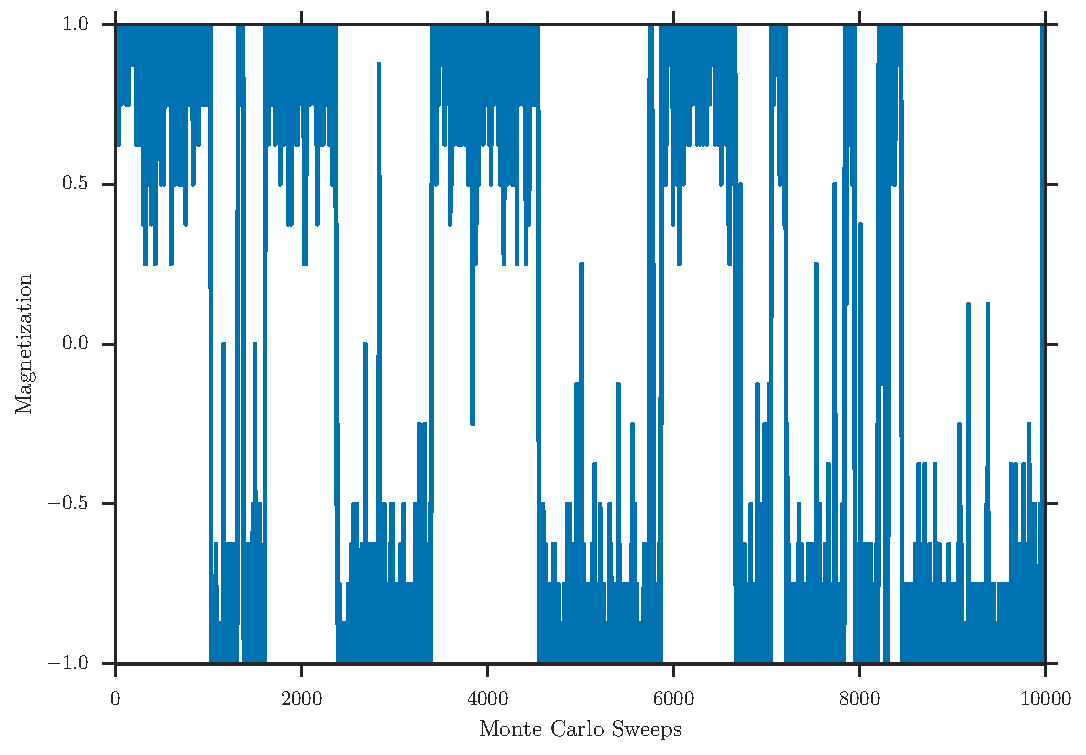
\includegraphics[width=\textwidth]{ising_4by4_magnetization_history.pdf}
	\caption{The magnetisation per spin of the Ising model. As the simulation runs (this simulation was done at \(T=2\) for a 4 by 4 system) the magnetisation oscillates.}
	\label{fig:ising_4by4_magnetization_history}
\end{figure}

These measurements are not statistically uncorrelated.
We define the autocorrelation function\cite{binney:1992}
\begin{equation}
	C(k) = \frac{\langle X_{\alpha_j} X_{\alpha_j+k} \rangle - \langle X_{\alpha_j} \rangle^2}{\langle X_{\alpha_j}^2 \rangle - \langle X_{\alpha_j} \rangle^2}
\end{equation}
with \(X_{\alpha_j}\) the values of \(X\) when the system is in state \(\alpha\) at time \(j\).
The autocorrelation function is 1 when k=0, meaning complete correlation between states, and is approximately 0 when \(k\) is large enough that the states are no longer correlated.
For long enough time scales the autocorrelation falls off as
\begin{equation}
	C(k) \propto e^{-k/\tau},
\end{equation}
where \(\tau\) is the typical time for this decay and is called the correlation time.
Because after a single correlation time the correlation function is still \(1/e\approx0.367\), it is best to sample once every 2\(\tau\) steps, when the correlation is only \(1/e^2\approx 0.135\).\cite{newman:1999}


\section{The Metropolis Algorithm}
The Metropolis algorithm, first published by Metropolis \textit{et al.} in 1953 \cite{metropolis:1953}, is a simple algorithm that was first used by its creators to study the dynamics of continuously displaceable hard spheres.
The algorithm is as follows\cite{binney:1992}:
\begin{enumerate}
	\item Choose a random site on the lattice.
	\item Flip the spin on this location and calculate the change in energy \(\Delta E\) associated with this spin-flip.
	\item Calculate the probability of accepting this move:
	\begin{equation}
		A =
		\begin{cases}
			e^{-\beta \Delta E}\ \ \ &\mathrm{if}\ \Delta E > 0 \\
			1 \ \ \ &\mathrm{if}\ \Delta E \leq 0
		\end{cases}
	\end{equation}
	\item Generate a random variable \(r\) in the interval \(\left[0, 1\right)\).
	\item Accept the move if \(r \leq A\). Otherwise leave the lattice as it was.
\end{enumerate}
The spin flip may also happen to a non-random spin simply by iterating over the rows and columns of the lattice. When studying only equilibrium dynamics, the two approaches are identical.\cite{landau:2015}
Ergodicity is satisfied because any state can be attained by flipping a sufficient number of single spins. Detailed balance is also satisfied.

To put a measure on the time elapsed in the simulation we define a sweep.
During a sweep every point on the lattice has been considered for flipping at least once.
Therefore a sweep consists of \(N\) of the steps described above.
The advantage of this is that time in a simulation can be measured independent of system size.\cite{newman:1999}

\begin{figure}[htb]
	\centering
	\begin{subfigure}[c]{0.2\linewidth}
		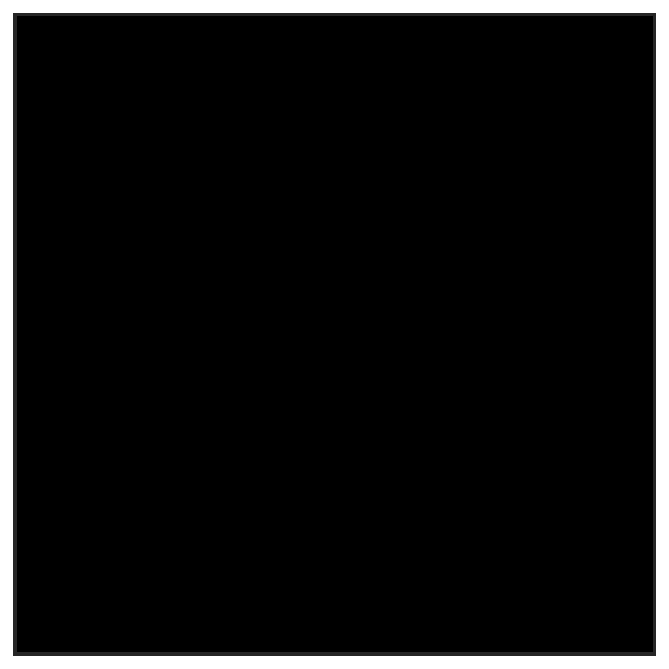
\includegraphics[width=\linewidth]{20160603124433_40_by_40_Lattice_step0.pdf}
	\end{subfigure}
	~
	\begin{subfigure}[c]{0.2\linewidth}
		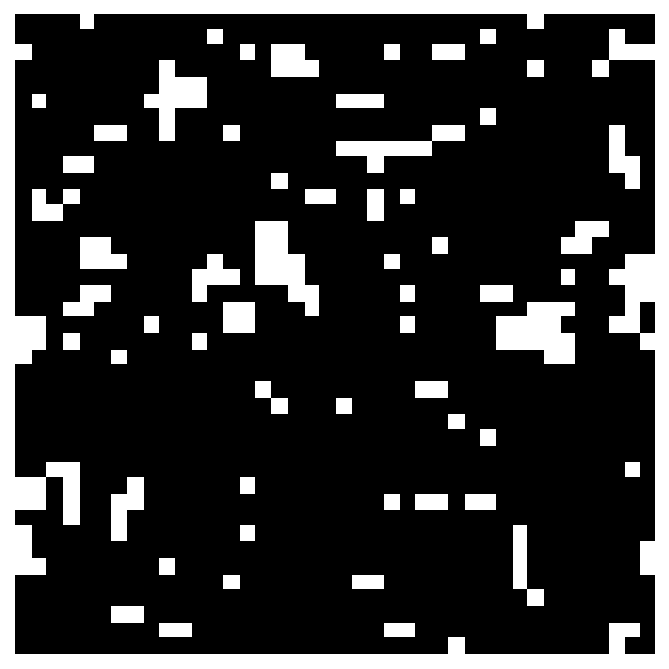
\includegraphics[width=\linewidth]{20160603125613_40_by_40_Lattice_step10.pdf}
	\end{subfigure}
	~
	\begin{subfigure}[c]{0.2\linewidth}
		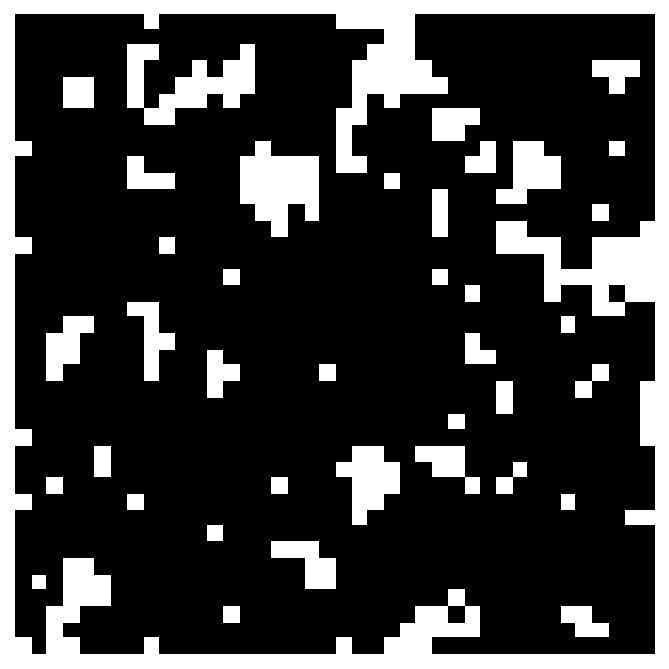
\includegraphics[width=\linewidth]{20160603125613_40_by_40_Lattice_step20.pdf}
	\end{subfigure}

	\begin{subfigure}[c]{0.2\linewidth}
		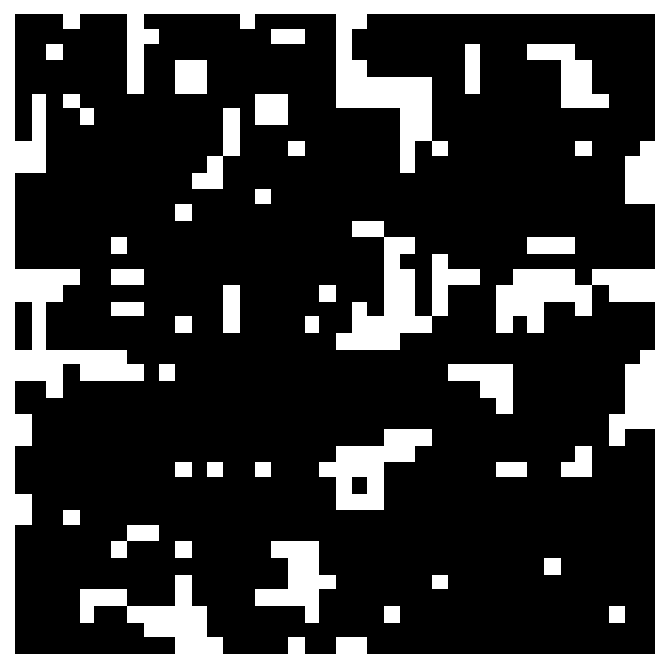
\includegraphics[width=\linewidth]{20160603125614_40_by_40_Lattice_step40.pdf}
	\end{subfigure}
	~
	\begin{subfigure}[c]{0.2\linewidth}
		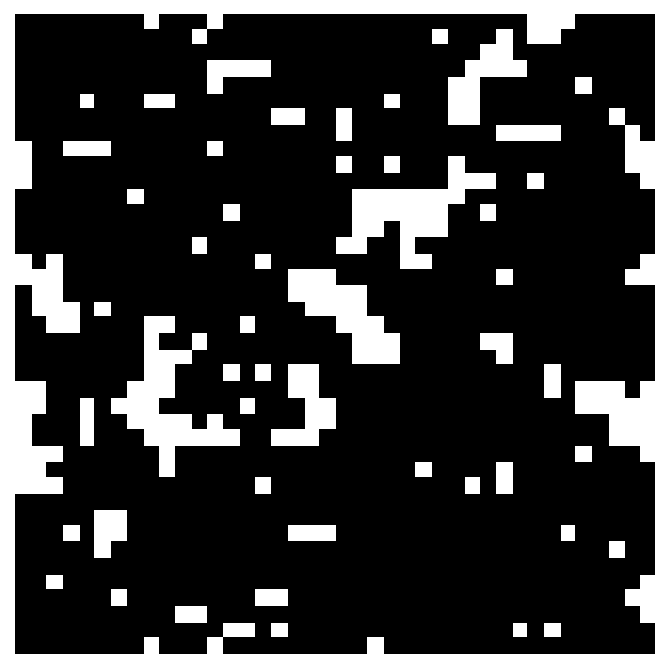
\includegraphics[width=\linewidth]{20160603125616_40_by_40_Lattice_step100.pdf}
	\end{subfigure}
	~
	\begin{subfigure}[c]{0.2\linewidth}
		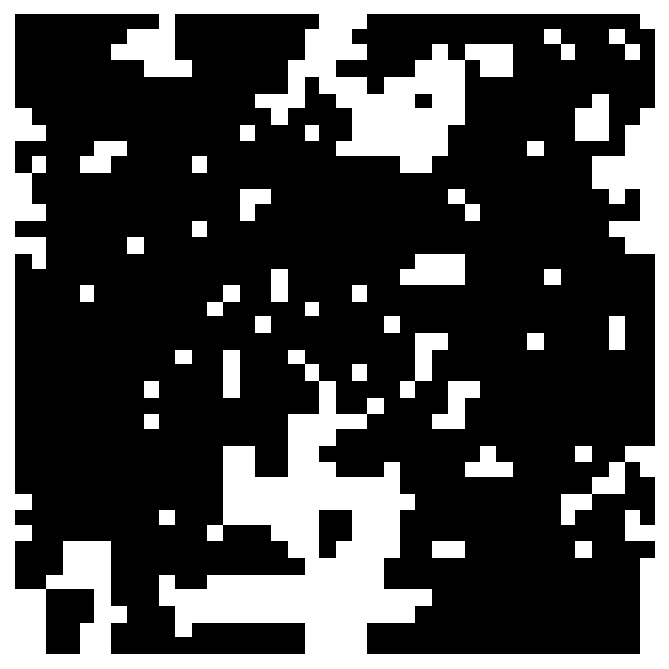
\includegraphics[width=\linewidth]{20160603125617_40_by_40_Lattice_step200.pdf}
	\end{subfigure}

	\begin{subfigure}[c]{0.2\linewidth}
		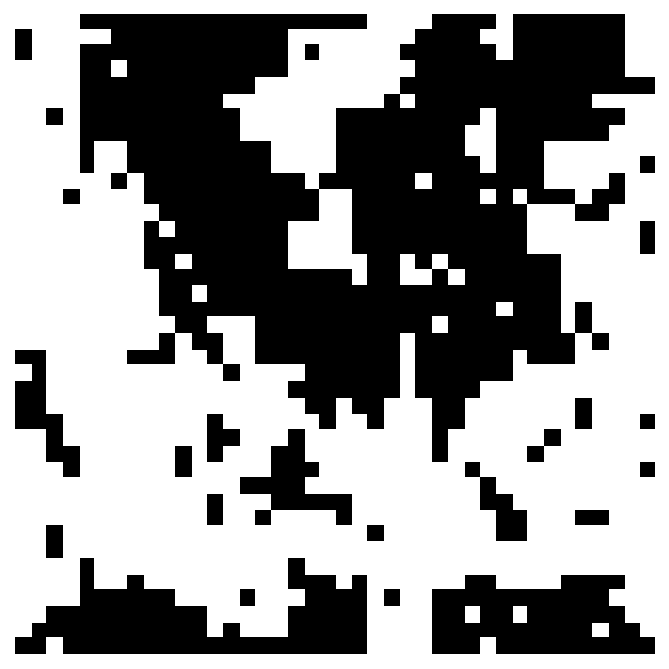
\includegraphics[width=\linewidth]{20160603125620_40_by_40_Lattice_step400.pdf}
	\end{subfigure}
	~
	\begin{subfigure}[c]{0.2\linewidth}
		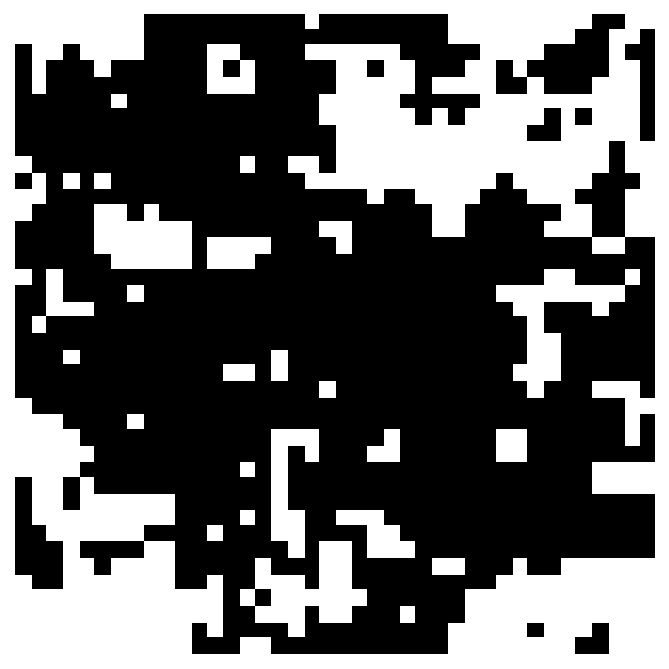
\includegraphics[width=\linewidth]{20160603125628_40_by_40_Lattice_step1000.pdf}
	\end{subfigure}
	~
	\begin{subfigure}[c]{0.2\linewidth}
		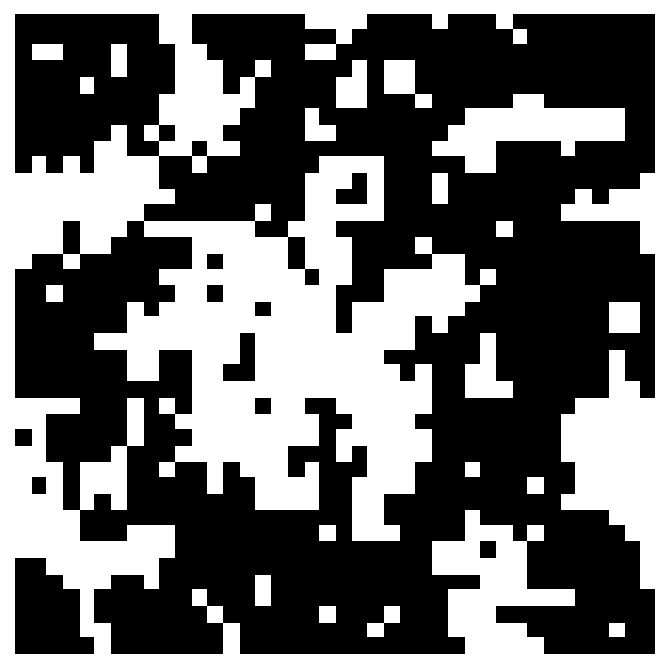
\includegraphics[width=\linewidth]{20160603125722_40_by_40_Lattice_step5000.pdf}
	\end{subfigure}
	\caption{A 40 by 40 Ising model lattice simulated using the Metropolis algorithm at \(T=2.4\) after 0, 10, 20, 40, 100, 200, 400, 1000	and 5000 sweeps. The simulation started in a completely ordered \(T=0\) state.}
\end{figure}

\subsection{Optimisations}
Especially for the Ising model simulated with the Metropolis algorithm some optimisation can be included in the simulation that have a large effect on runtime.
The exponentials needed for the acceptance ratio can be pre-calculated since there are (in two dimensions) only 5 possible different ways in which the neighbours are oriented:
all aligned, 3 aligned, etcetera.
Because the exponentials require costly floating point operations, caching those values gives a significant speed increase compared to recalculating them at every step.

For the energy of the Ising model simulated with the Metropolis algorithm there is a trick that allows for much quicker computation of the energy difference than explicitly using the Hamiltonian, which requires as many calculations as there are bonds in the system, a number that scales with \(N\).
The difference in energy between two states \(\mu\) and \(\nu\) is
\begin{align}
	E_{\nu} - E_{\mu} &= -J \sum_{\langle ij \rangle} \sigma_i^{\nu} \sigma_j^{\nu} + J \sum_{\langle ij \rangle} \sigma_i^{\mu} \sigma_j^{\mu}\\
	&= -J \sum_{\substack{i\ \mathrm{nearest}\\ \mathrm{neighbour\ to}\ k}} \sigma_i^{\mu}\left(\sigma_k^{\nu} - \sigma_k^{\nu}\right)
\end{align}
The term in brackets can only be -2 or +2, dependent on the value of the spin \(k\) to be flipped before the flip.
Thus \(\sigma_k^{\nu} - \sigma_k^{\nu} = -2 \sigma_k^{\mu}\) and
\begin{equation}
	E_{\nu} - E_{\mu} = 2 J \sigma_k^{\mu} \sum_{\substack{i\ \mathrm{nearest}\\ \mathrm{neighbour\ to}\ k}} \sigma_i^{\mu}
\end{equation}
This expression depends only on the neighbours of the spin that is to be flipped and can be calculated before a spin is flipped.
Using that \(E_{\mu} = E_{\nu} + \Delta E\) we only have to calculate the energy using the hamiltonian once at the start, and then update the energy after every step with the change in energy.
A similar trick can be used for the magnetisation, where the change in magnetisation can be shown to be \(\Delta M = 2\sigma_k^{\mu}\).\cite{newman:1999}


\subsection{Critical Slowing Down}\label{sec:critical_slowing_down}
The Metropolis algorithm is very simple but does have one major drawback.
Close to the phase transition, the correlation time diverges.
This is because there the correlation time goes like
\begin{equation}
	\tau \propto \xi^z,
\end{equation}
where \(z\) is called the critical dynamical exponent and is different for each algorithm and system.
During critical slowing down in single spin-flip algorithms the correlation length diverges (up to the system size \(L\)) and islands are formed in which all spins point in the same direction.
A statistically independent configuration would need to have a significant chance of flipping the spins in such an island.
However, flipping a spin whose neighbours are pointing in the same direction is energetically unfavorable and thus has a suppressed acceptance probability.
Therefore the correlation time becomes large and the simulation would have to run for a long time to create enough statistically independent measurements,\cite{binney:1992} especially since at \(T_c\) \(\xi = L\), meaning that it would quickly become impractical to simulate large systems.
For the two dimensional Ising model simulated with the  Metropolis algorithm the dynamic critical exponent has been measured to be \(z=2.1665(12)\).\cite{nightingale:1996}

\section{The Wolff Algorithm}
The Wolff algorithm significantly improves in the area of critical slowing down, having a dynamic critical exponent of \(z=0.25(2)\)\cite{barkema:1991}.
It was first proposed by Wolff in 1989\cite{wolff:1989}, and works by not flipping single spins, but building clusters of spins pointing in the same direction and flipping those en masse.
The Wolff algorithm goes as follows\cite{landau:2015,newman:1999}:
\begin{enumerate}
	\item Choose a random site on the lattice \(i\)
	\item\label{item:wolff_step_two} Look at the neighbours of \(i\). If a neighbour \(j\) has the same spin as \(i\), add it to the cluster with probability \(P = 1 - e^{-2\beta J}\).
	\item Repeat step \ref{item:wolff_step_two} for spin \(j\) until no more spins can be added to the cluster.
	\item Flip the entire cluster.
\end{enumerate}
If a spin was considered during a previous step but not added to the cluster, this spin may be reconsidered for future steps.
Spins that are already part of the cluster are not added again.
The algorithm fulfills the condition of detailed balance because there is always a non-zero chance that a cluster will consist of only a single spin.
A succession of such single spin-flip clusters can reach any state. Detailed balance is also satisfied.
Given the much smaller critical exponent for the Wolff algorithm compared to the Metropolis algorithm, critical slowing down is mostly absent.

To compare the correlation times of the Metropolis and Wolff algorithm, we need to properly define the correlation time of the Wolff algorithm.
A single step will create a cluster that could corresponds to a great many steps of the Metropolis algorithm.
On average a Wolff cluster will cover a fraction of the lattice \(\langle n \rangle / L^2\). (See \cref{fig:wolff_cluster_size}. As the temperature increases, the probability to add a spin to the cluster decreases, meaning average cluster size decreases.)
This corresponds to a single sweep of the lattice in a Metropolis simulation.
The correlation time is then
\begin{equation}
	\tau = \tau_{\mathrm{steps}} \frac{\langle n \rangle}{L^2}.
\end{equation}
This is especially important in the high temperature regime, where many single-spin cluster will form.
Without the correction the correlation time would be too large.\cite{newman:1999}
Comparing correlation time for the Ising model between the Metropolis and Wolff algorithm, it is found that there is indeed a marked difference.
For Wolff simulations the correlation time of the absolute magnetisation is always of order 1, even for lattices as large as 40 by 40.
In contrast Metropolis simulations show a correlation time at the critical point of \(\sim 12\) sweeps, for even modest sized 10 by 10 lattices.


\begin{figure}[htb]\label{fig:wolff_cluster_size}
	\centering
	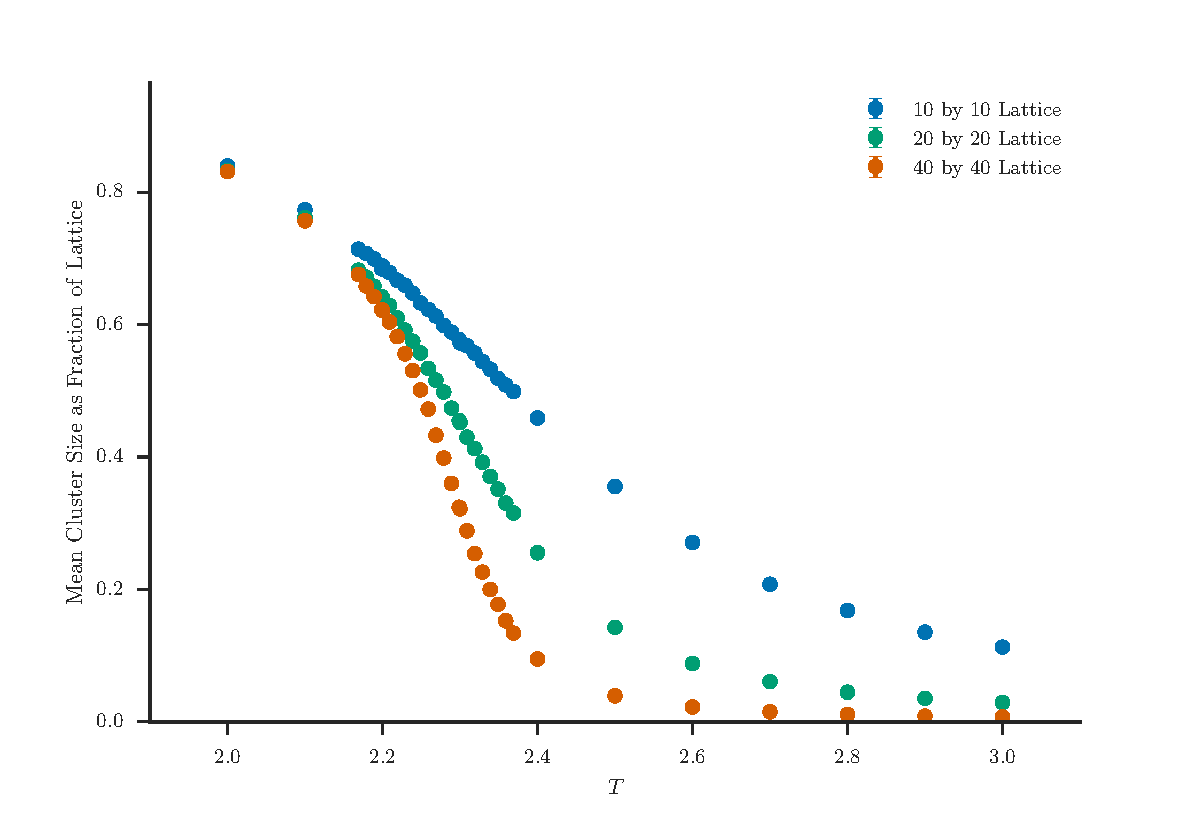
\includegraphics[width=\textwidth]{wolff_mean_cluster_size_as_fraction_of_lattice.pdf}
	\caption{The mean size as a fraction of the lattice of clusters generated with the Wolff method. During the simulation the temperature varied from 2 to 3 in steps of 0.1, with a higher resolution of 0.01 from 2.169 to 2.369. The error bars are too small to see.}
\end{figure}

\subsection{Generalising Algorithms to the Potts Model}
Both the Metropolis and Wolff algorithm can be easily generalised to the q-state Potts model.
For the Metropolis algorithm we again pick a random spin \(s\) in state \(i\).
We then pick a new state \(j\) from the remaining \(q-1\) possible state for that spin such that \(s_i \neq s_j\).
After that we proceed as described earlier.
Just like for the Ising model the algorithm satisfies the ergodicity and detailed balance conditions.
For large \(q\) more efficient algorithms exist, but for \(q=3\) Metropolis works fine.
There is still critical slowing down, with a dynamic critical exponent of \(z=2.198(8)\)\cite{newman:1999} or \(z=2.171(62)\).\cite{fan:2007}

Given this slowing in the Potts model cluster algorithms are again more appropriate when investigating the area around the phase transition.
The generalised Wolff algorithm proceeds exactly the same as in the Ising case, with the only difference being that the probability to add a spin to the cluster has become \(P_{add} = 1 - e^{-\beta J}\).
We can see where this factor of 2 comes from by considering the \(q=2\) Potts model.
The Hamiltonian is still
\begin{equation}
	H = -J\sum_{\langle i j \rangle} \delta(\sigma_i, \sigma_j),
\end{equation}
but for the two-state model we can rewrite this as
\begin{equation}
	H = -\frac{1}{2} J \sum_{\langle i j \rangle} 2 \left(\delta(\sigma_i, \sigma_j\right) - \frac{1}{2}) - \sum_{\langle i j \rangle} \frac{1}{2}J.
\end{equation}
These expressions are the same except for a constant, since for \(\sigma_i = \sigma_j\) we have \(2 (\delta(\sigma_i, \sigma_j) - \frac{1}{2}) = +1\) while it is -1 otherwise.
We therefore have an interaction energy \(\frac{1}{2}J\) instead of \(J\), explaining the change in the addition probability.
This algorithm again satisfies detailed balance and ergodicity.\cite{newman:1999}
The dynamic critical exponent is \(z=0.60(2)\), again a significant improvement over the Metropolis algorithm.


\chapter{Analysis of Monte Carlo Simulations}
\section{Statistics}
Now that we have obtained measurements for the energy and magnetisation of the Ising and Potts models, we need to find a way to make these measurements statistically uncorrelated, since the state of a lattice after a single algorithm sweep may not be very different compared to the state before.
Because typical methods for error calculation assume uncorrelated samples, those methods do not work.
We can calculate the autocorrelation times, and only sample once every two correlation times, but an easier and quicker approach is the Binning method.

\subsection{Binning}

The Binning method creates uncorrelated sequences of data from a given correlated output.
Consider an original data set \(A_i^{(0)}\) with \(i = 1, \ldots N\) and \(N\) the number of data points in the original set.
Iteratively combine two consecutive data points into a bin according to
\begin{equation}
	A_i^(l) = \frac{1}{2} \left(A_{2i-1}^{(l-1)} + A_{2i}^{(l-1)} \right) \mathrm{\ \ \ with \ \ \ } i = 1, \ldots, N_l = \frac{N}{2^l},
\end{equation}
with \(l\) the current binning step.
The average in each bin is less correlated with every step while the mean remains the same.
The error on a quantity for a given binning step is
\begin{equation}
	\label{eq:basic_error}
	\Delta A^{(l)} = \sqrt{\frac{\mathrm{Var}(A^{(l)})}{N_l}}.
\end{equation}
As the binning progresses the error for each step converges to the actual error, meaning that in a plot the errors tend to a plateau (\cref{fig:binning_error_convergence}).
This method can then be used to calculate the error on the energy, magnetization and any higher order data such as \(E^2\).

From the binning method we can also determine the autocorrelation time:\cite{corboz}
\begin{equation}
	\tau = \frac{1}{2} \left[\left( \frac{\Delta A^{(l_{max})}}{\Delta A^{(0)}} \right)^2- 1 \right]
\end{equation}
\begin{figure}[htb]
	\centering
	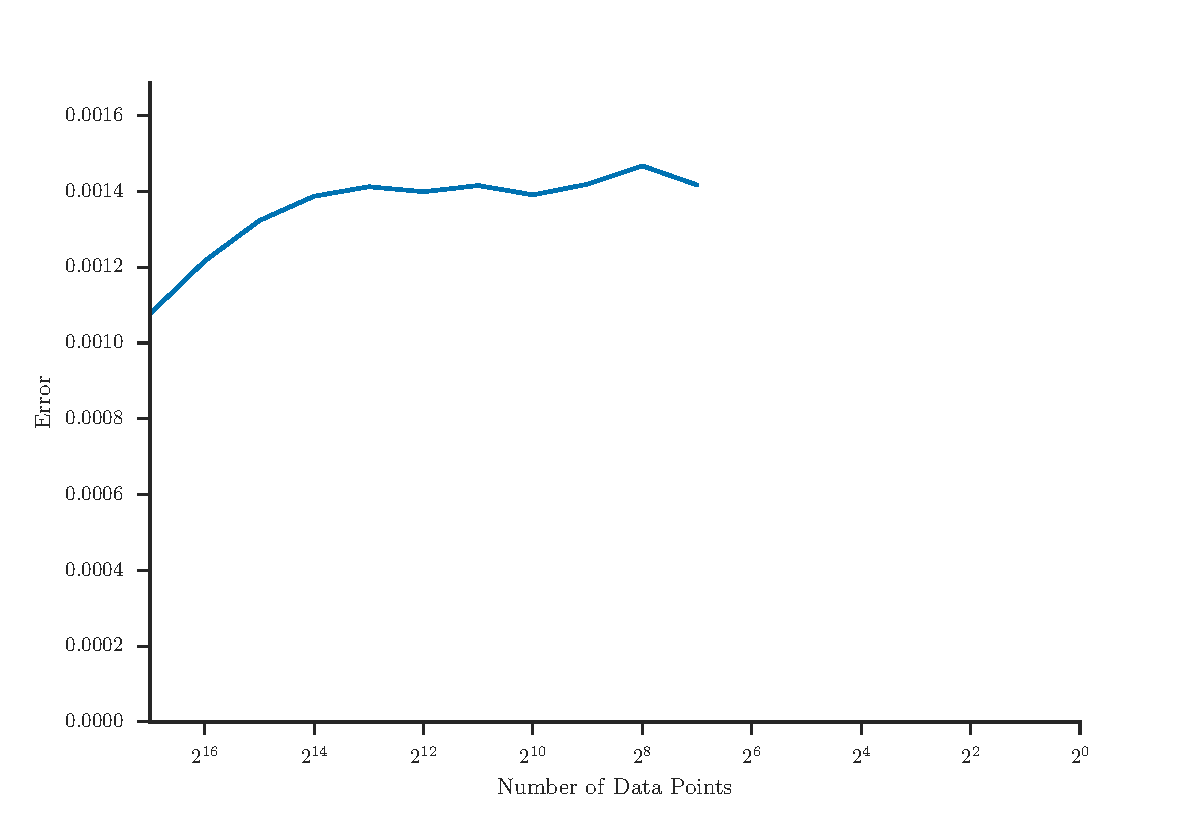
\includegraphics[width=\textwidth]{ising_metropolis_energy_per_site_error_binning.pdf}
	\caption{The error for the energy per site as a function of the data size. As the binning progresses the error tends to a plateau. A 10 by 10 Ising model was simulated at a temperature of 2, thermalised for 5000 sweeps and then measured for 65536 sweeps.}
	\label{fig:binning_error_convergence}
\end{figure}

\subsection{Bootstrap and Jackknife}
Other interesting values we would like to know are functions of measured values.
These include the heat capacity \(c\) and magnetic susceptibility \(\chi\):
\begin{align}
	c &= \frac{\beta^2}{N} \left(\langle E^2 \rangle - \langle E \rangle^2 \right), \\
	\chi &= \beta N \left( \langle m^2 \rangle - \langle m^2 \rangle \right).
\end{align}
These quantities are not defined at a single instant of the simulation, but instead depend on time averages of the energy or magnetisation.
Note that binning has to happen for both \(E\) and \(E^2\) separetly when statistically independent samples are created.
One way to calculate the error on these values is to run the same simulation a large number of times and calculate the error from the calculate errors.
Given the long running times of Monte Carlo simulations this is not always practical.

To still be able to calculate errors on the quantities we use resampling methods.
The first method that was used is the bootstrap method.
For concreteness we consider the specific heat.
Given a list of \(n\) measurements of the energy (and the energy squared), we randomly choose \(n\) values, allowing duplicates.
Strictly speaking these measurements should be independent, but for the bootstrap method this does not matter.
We can simply use measurements made after every sweep of the lattice.
With the \(n\) samples we calculate the desired quantity.
Then we repeat the random sampling a number of times (1000 should be enough).
With those 1000 values of the heat capacity, we can use basic methods to calculate errors, such as \cref{eq:basic_error}.\cite{newman:1999}

We can also used the jackknife method.
Here we do need statistically uncorrelated samples.
With these samples we calculate the heat capacity \(c_0\).
Then, we calculate the heat capacity \(c_i\) for which we took out the \(i\)-th measurement from our data set.
Replacing it we next remove the \(i+1\)-th measurement, and so on.\cite{newman:1999}
The error becomes\cite{corboz}
\begin{equation}
	\Delta c = \sqrt{M-1}\left( \frac{1}{M} \sum_{i=1}^M \left[c_i^2 - c^2\right] \right)^{1/2},
\end{equation}
with \(M\) the number of statistically independent measurements.

Following the advice of Landau and Binder \cite{landau:2015}, when different methods give different errors we use the largest error calculated.

\section{The Binder Cumulant}
Given these statistically independent measurements, one thing we may like to find is the critical temperature.
Unfortunately we cannot determine this simply by looking at the order parameter of a system and when it becomes zero, because the finite size of the simulated lattices precludes a sharp phase transition.
We can however define the Binder cumulant\cite{binder:1981b}
\begin{equation}
	U_4 = 1 - \frac{\langle m^4 \rangle}{3 \langle m^2 \rangle^2},
\end{equation}
which for \(L \to \infty\) becomes \(2/3\) for \(T \to 0\) and 0 for \(T \to \infty\).\cite{landau:2015}
At the critical temperature \(U_4\) has the same value independent of the lattice size.
Therefore the critical temperature can be found by plotting the binder cumulant for different lattice sizes and looking for the intersection (as seen in \cref{fig:ising_binder_cumulant}).
\begin{figure}[htb]
	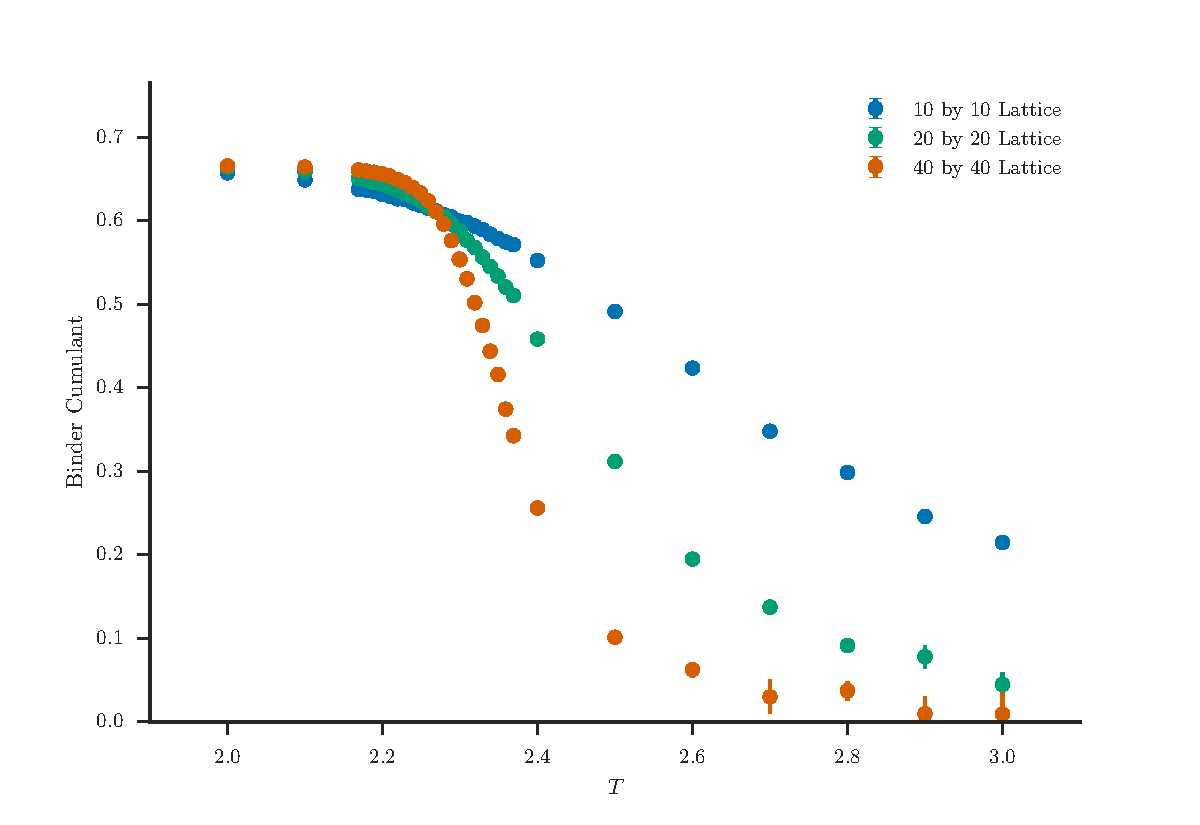
\includegraphics[width=\textwidth]{wolff_binder_cumulant.pdf}
	\caption{The Binder cumulant for the Ising model at three different lattice sizes. The critical point occurs at approximately \(T = 2.26\). The values were acquired by simulation the lattice using the Wolff algorithm and running 65536 steps after equilibration. During the simulation the temperature was varied from 2 to 3 in steps of 0.1, with a higher resolution from 2.169 to 2.369 in steps of 0.01. The error bars are too small to see in this plot.}
	\label{fig:ising_binder_cumulant}
\end{figure}

\section{Finite Size Scaling}
To extract the critical exponents for different models, one way to proceed is to use finite size scaling.
The advantage of this method is that \(T_c\) does not need to be known in advance, although if a value has already been determined using the Binder cumulant, this can also be used.

We derive finite size scaling for the magnetic susceptibility.
Close to the critical temperature we have \(\chi \propto \abs{t} ^{-\gamma}\) with \(t = (T-T_c) / T_c\) (\cref{eq:chi_divergence}).
We also know that for the correlation length \(\xi \propto \abs{t}^{-\nu}\) in this region (\cref{eq:correlation_length}).
Therefore we can write \(\chi \propto \xi^{\gamma /\nu}\).

The finite size of simulated systems introduced a cutoff for the correlation length equal to the system size \(L\), also cutting off the divergence of the susceptibility.
If \(\xi\) is the correlation length of the infinite system, the cutoff occurs when \(\xi > L\).
For \(\xi \ll L\) \(\chi\) should be the same as in the infinite system.
We can then write for \(\chi\):
\begin{equation}\label{eq:finite_size_chi}
	\chi = \xi^{\gamma/\nu} \chi_0(L/\xi).
\end{equation}
where \(\chi_0\) has the properties
\begin{align}
	\chi_0(L/\xi) &= \mathrm{constant}\ \ \ \ \mathrm{for}\ L \gg \xi,\\
	\chi_0(L/\xi) &\propto (L/\xi)^{\gamma/\nu}\ \ \ \ \mathrm{as}\ L/\xi \to 0.
\end{align}
Because we do not know the correlation length of the infinite system it is more useful to define
\begin{equation}
	\tilde{\chi} = (L/\xi)^{-\gamma} \chi_0((L/\xi)^{\nu}),
\end{equation}
with which we can rewrite \cref{eq:finite_size_chi} to get
\begin{equation}
	\tilde{\chi}(L^{1/\nu}t) = L^{-\gamma/\nu}\chi.
\end{equation}
We call \(\tilde{\chi}\) the scaling function.
All dependence on system size has been extracted from the scaling function, meaning that its value is the same for all \(L\) when close to the critical temperature.
Given a set off data for the susceptibility, we can calculate the scaling function for different \(\gamma\), \(\nu\) and \(T_c\).
If the values are correct, the data collapses onto a single curve around \(t=0\) when plotted (\cref{fig:ising_data_collapse}).
For the specific heat and magnetisation similar equations can be derived\cite{newman:1999}:
\begin{align}
	\widetilde{c}(L^{1/\nu}t) &= L^{-\alpha/\nu} c, \\
	\widetilde{m}(L^{1/\nu}t) &= L^{\beta/\nu} m.
\end{align}

If \(T_c\) is known, simulations for different system sizes at \(T_c\) can be performed and a log-log plot of the data can be created to determine ratios of critical exponents.
For this we use that at the critical point \(L = \xi\) and the susceptibility scales as \(\chi \propto L^{\gamma/\nu}\).
Then the value of the susceptibility scales with system size as
\begin{equation}
	\log(\chi) = \gamma/\nu \log(L) + \mathrm{constant}.
\end{equation}
Plotting the values, the slope of the line passing through the points, which can be determined by a linear fit, gives the ratio \(\gamma/\nu\) (see \cref{fig:ising_magnetizabilities_loglog_plot}).\cite{corboz}

\begin{figure}[htb]
	\centering
	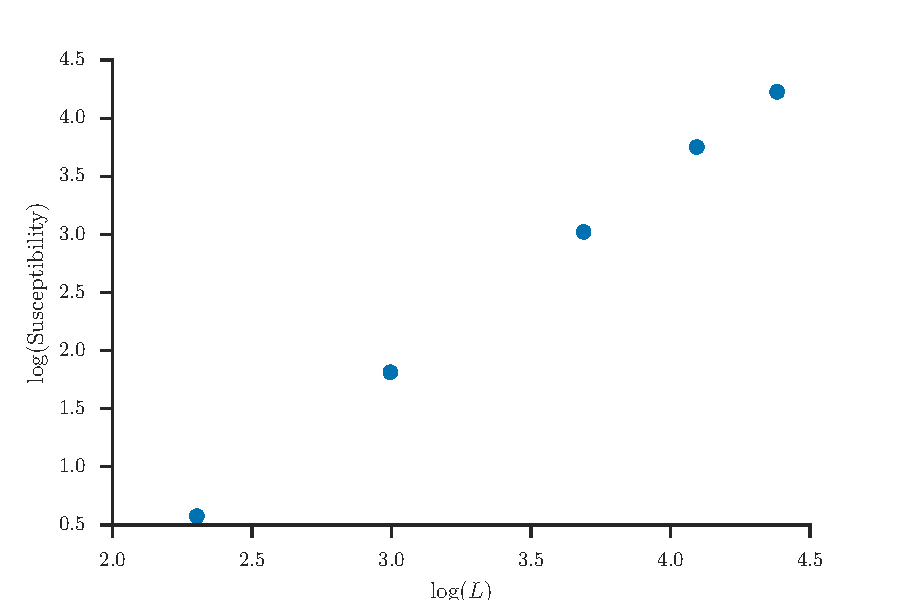
\includegraphics[width=\textwidth]{ising_magnetizabilities_loglog_plot.pdf}
	\caption{Log-Log plot of the magnetic susceptibility of the Ising model at \(T_c\) for systems of size 10, 20, 40, 60 and 80.}
	\label{fig:ising_magnetizabilities_loglog_plot}
\end{figure}

\begin{figure}[htb]
	\centering
	\begin{subfigure}{\textwidth}
		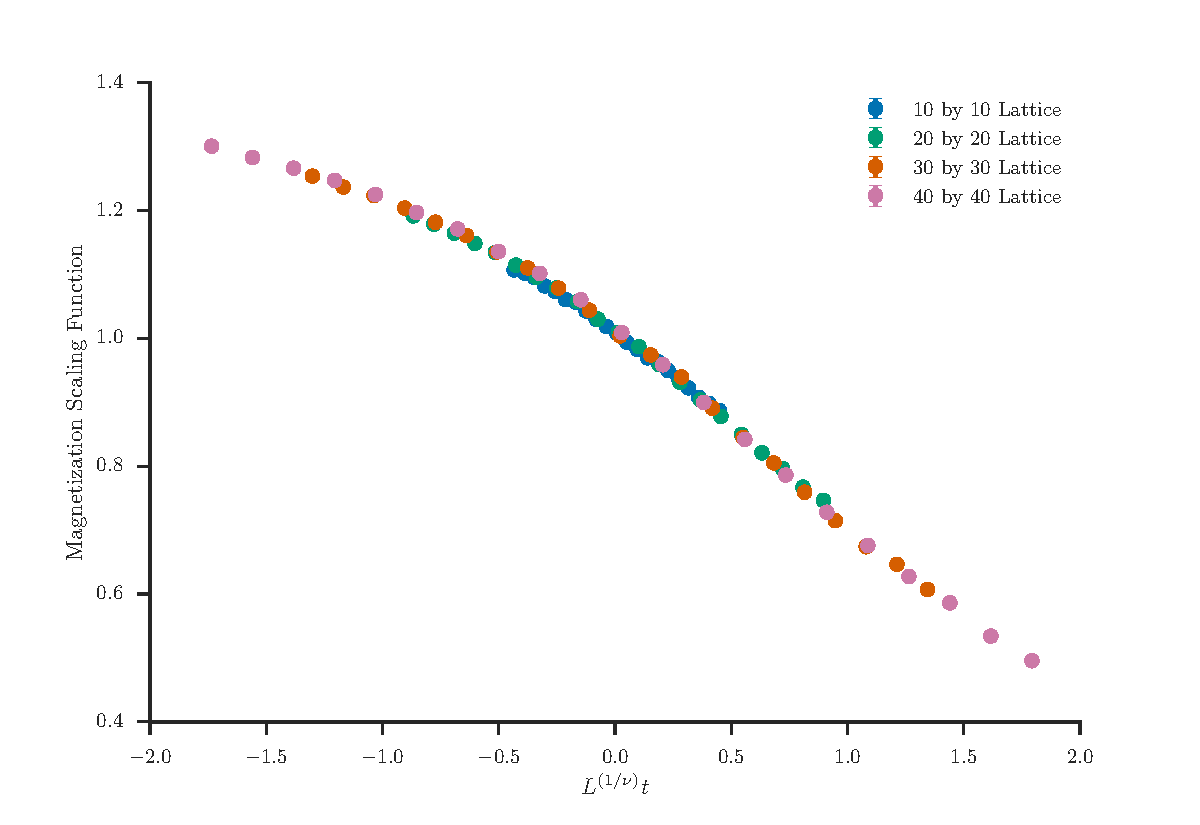
\includegraphics[width=\textwidth]{ising_magnetization_exact_data_collapse.pdf}
	\end{subfigure}

	\begin{subfigure}{\textwidth}
		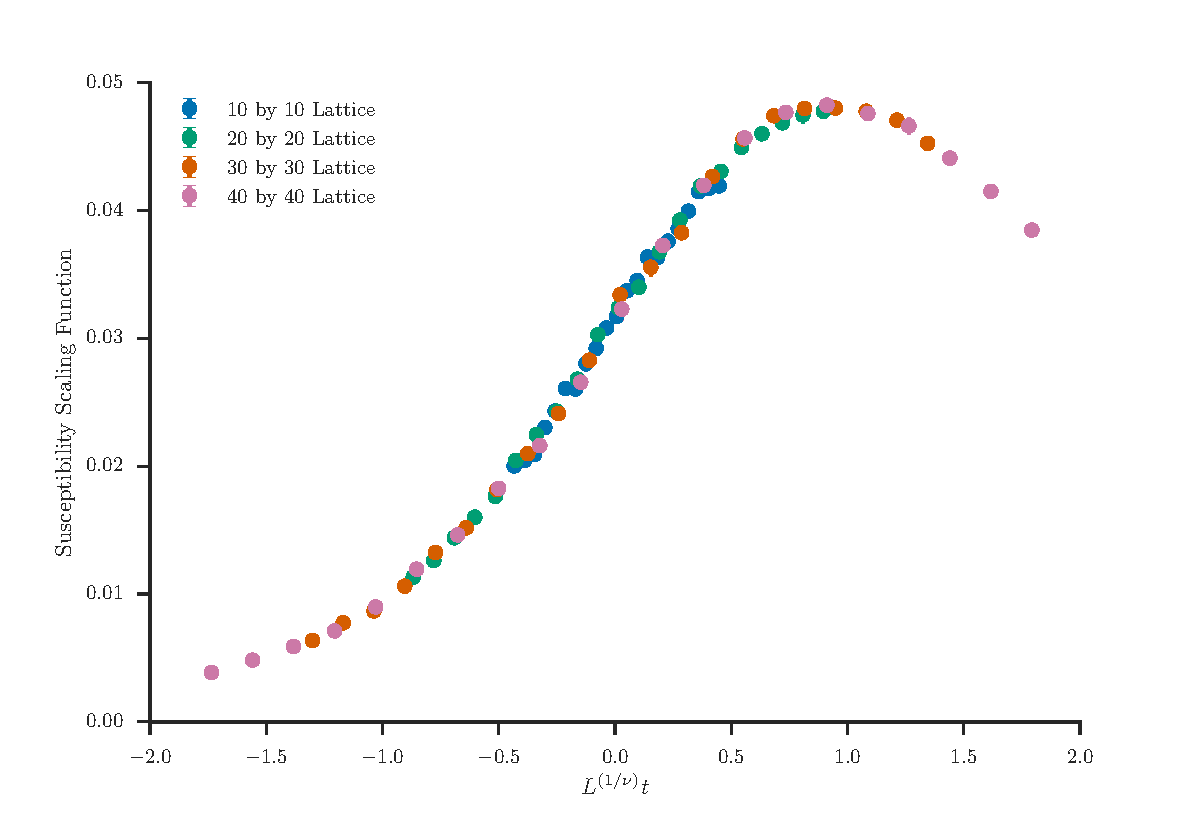
\includegraphics[width=\textwidth]{ising_susceptibility_exact_data_collapse.pdf}
	\end{subfigure}
	\caption{Finite size scaling data collapse for the magnetisation and the magnetic susceptibility of the Ising model. The exact values for the exponents \(\gamma = 7/4\), \(\nu=1\) and \(\beta=1/8\) were used.}
	\label{fig:ising_data_collapse}
\end{figure}


\chapter{Results}

All results were obtained from simulations of the Wolff algorithm around the critical point.
Runs consisted of 10000 equilibration sweeps, followed by 65536 measurement sweeps.
For the Wolff algorithm a sweep was defined as constructing a single cluster.
\todo{Indicate how reliable your results are}

\section{The Ising Model at Criticality}

The critical temperature of the Ising model in two dimensions in zero field was determined by finding the intersection of the Binder cumulant for lattices of sizes 10, 20, 30 and 40 (\cref{fig:ising_binder_cumulant}).
First a simulation in the range 2 to 3 with steps of 0.1 was performed to roughly locate the critical point.
A more fine-grained simulation from 2.169 to 2.369 with a resolution of 0.01 was performed afterwards.
The critical temperature was determined to be 2.267(2).
The critical temperature agrees well with Onsager's result of 2.269\cite{onsager:1944}, as well as those of Ghaemi \textit{et al.} of \(T_c = 2.2691(5)\)\cite{ghaemi:2001}.

The intersection of the Binder cumulants was determined by linearly extrapolation between two consecutive data points and trying to find an intersection of those lines between consecutive lattice sizes.
The average of the different intersection points was taken for the value.
To determine the error on the estimate intersections were also found for the data points with their respective errors added and subtracted.

Using Log-Log plots the ratio of critical exponents was determined.
The ratio \(\beta/\nu\) was determined by a linear fit of the magnetisation and was determined as 0.125(1).
From a fit of the susceptibility (\cref{fig:ising_magnetizabilities_loglog_plot}), we found \(\gamma/\nu = 1.758(8)\).
Both of those values agreed well with the exact values of \(\beta/\nu = 0.125\) and \(\gamma/\nu = 1.75\).

With the determined critical temperature and ratio of critical exponents a data collapse was performed.
By having \(\nu\) run over a range of 0.01 to 1 in steps of 0.01, while determining the other critical exponent using the ratio, a data collapse was performed.
As suggested by Sandvik\cite{sandvik:2011}, the quality of the data collapse was assessed using a chi-least-squares test.
A polynomial of degree 6 was fitted to the data in the range where most data points fell after scaling, which was in the interval \(L^{1/\nu}t \in [-1, 1]\).

\begin{table}[htb]
	\centering
	\renewcommand{\arraystretch}{1.5}
	\begin{tabular}{l | c c c c c c}
		\hline
		& \(\alpha\) & \(\beta\) & \(\gamma\) & \(\eta\) & \(\nu\) & \(\delta\) \\\hline
		Exact & 0 & \(\frac{1}{8}\) & \(\frac{7}{4}\) & \(\frac{1}{4}\) & 1 & 15 \\
		\(\beta/\nu\) & 0.075(13) & 0.1204(8) & 1.683(14) & 0.250(2) & 0.962(6) & 15(2.8) \\
		\(\gamma/\nu\) & 0.002(2) & 0.121(2) & 1.756(3) & 0.2424(5) & 0.999(1) & 15.5(14.6)\\\hline
	\end{tabular}
\end{table}
The value for \(\delta\) calculate using \(\gamma/\nu\) has such a large error because, during error propagation the ration \(\Delta \alpha / \alpha\) is approximatly 1. The error on this value can therefore not be regarded as sensible.

With the ratio \(\alpha / \nu\) it is only possible to determine \(\alpha\) and \(\nu\), because the system of equations consisting of the scaling laws after filling in the values of \(\alpha\) and \(\nu\) is a system of three equations with 4 unknowns and therefore underdetermined.
The log-log plot of the specific heat at criticality gave a ratio \(\alpha / \nu = 0.287(17)\).
The collapse for the specific heat gave very poor results and gave values of \(\alpha = 0.287(5)\) and \(\nu =1\).
For \(\nu\) no error could be determined because for all fits \(\nu = 1\) gave the best results.

It was also the case that while iterating over different values of \(\nu\) the upper bound for \(\nu\) was always determined to give the best fit, even though values of \(\nu\) larger than 1 are unphysical in this case.
For the fits which used \(\beta/\nu\) and \(\gamma/\nu\) the physical exponents remained the same no matter what the upper bound for \(\nu\) was.


\begin{figure}
	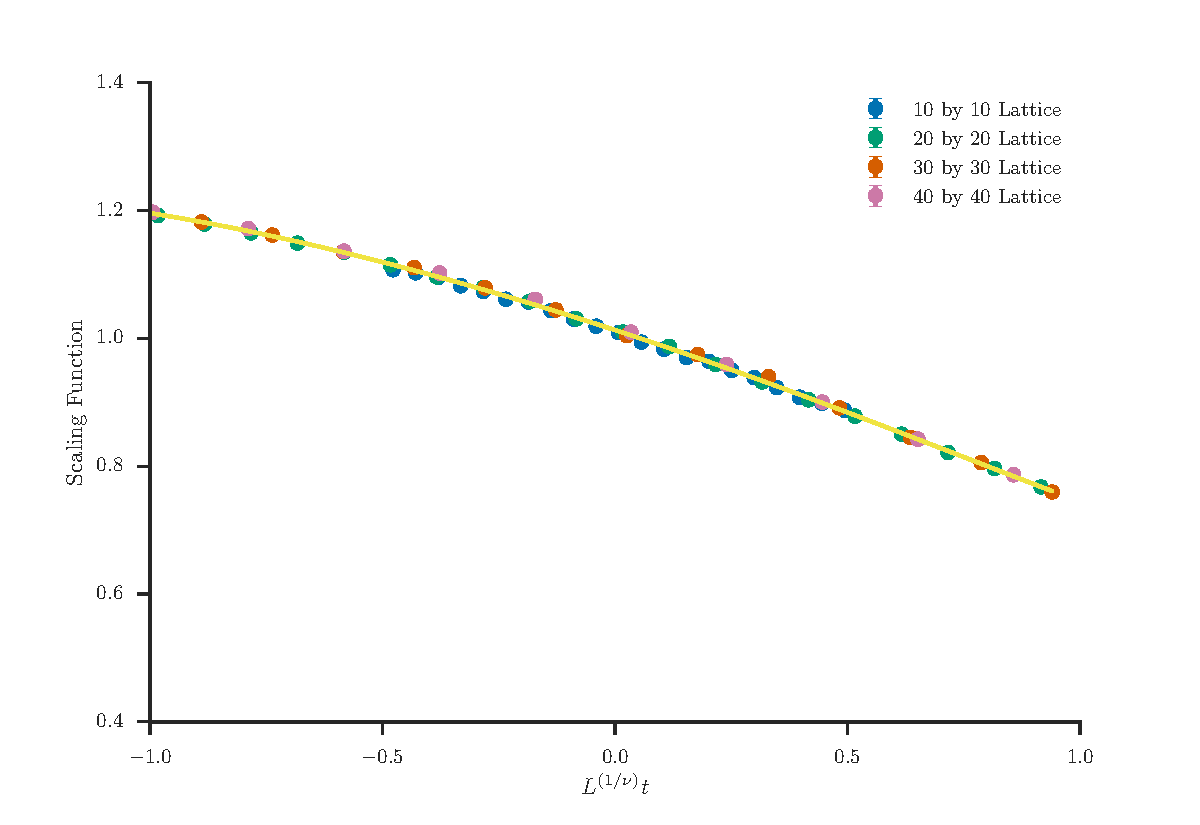
\includegraphics[width=\textwidth]{ising_beta_over_nu_data_collapse.pdf}
	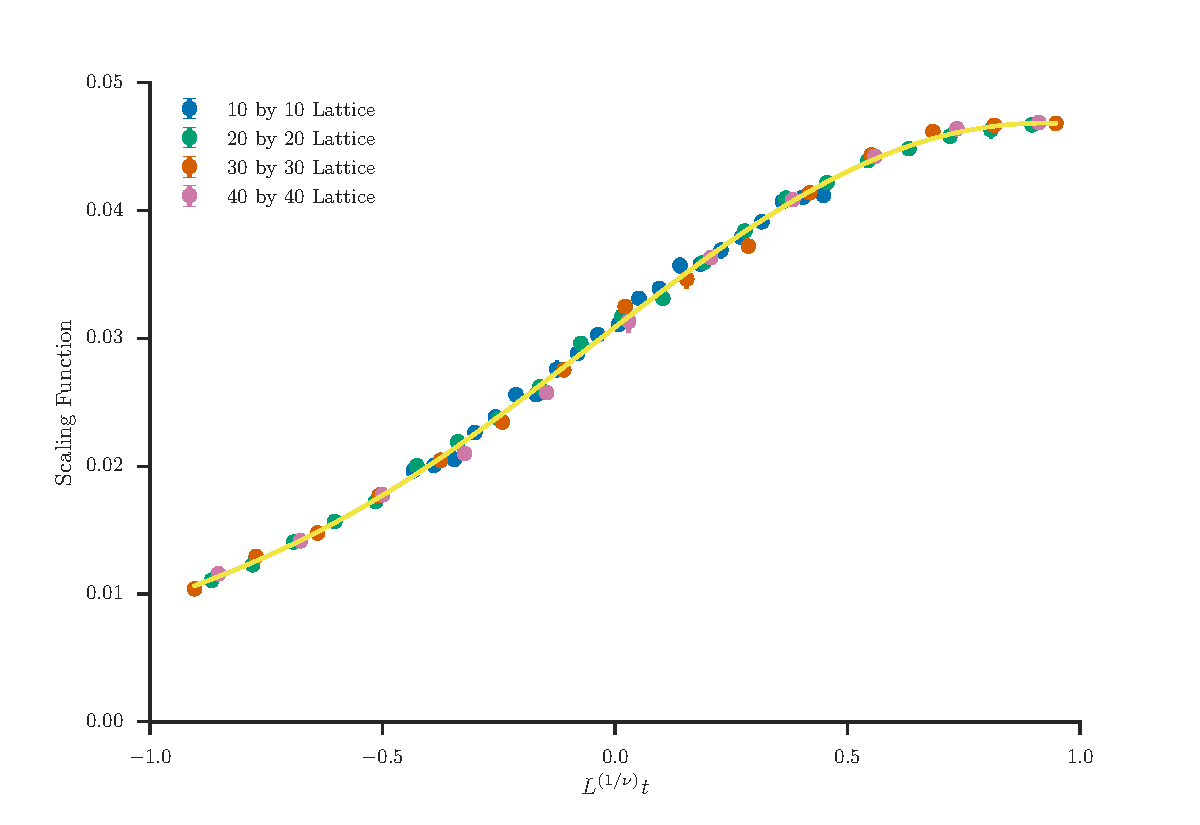
\includegraphics[width=\textwidth]{ising_gamma_over_nu_data_collapse.pdf}
	\caption{Data collapses of the magnetisation and magnetic susceptibility, using a chi-least-squares method to determine the goodness of fit (yellow line). The images shown represented the best collapse that could be performed.}
	\label{fig:ising_chi_data_collapse}
\end{figure}


\section{The Potts Model at Criticality}

For the 3-state Potts model in two dimensions and zero-field the critical temperature was found to be \(T_c=1.020(22)\) using Binder intersection at \(L = 10, 20, 40\).

This is in reasonable agreement with the result of Ghaemi \textit{et al.}\cite{ghaemi:2001} (\(T_c=0.9950(1)\)), as well as those of Fan \textit{et al.}\cite{fan:2007} of \(T_c = 0.9968(20)\).

\begin{table}[htb]
	\begin{adjustbox}{center}
		\centering
		\renewcommand{\arraystretch}{1.5}
		\begin{tabular}{l | c c c c c c}
			\hline
			& \(\alpha\) & \(\beta\) & \(\gamma\) & \(\eta\) & \(\nu\) & \(\delta\) \\\hline
			Den Nijs (1979)\cite{nijs:1979,baxter:1989} & \(\frac{1}{3}\) & \(\frac{1}{9}\) & \(\frac{13}{9}\) & \(\frac{4}{15}\) & \(\frac{5}{6}\) & 14 \\
			Blöte (1981)\cite{blote:1981} & \(\sim\frac{1}{3}\) & & & & & \(\sim14\)\\
			Fan (2007)\cite{fan:2007} & 0.396(66) & 0.108(4) & 1.416(62) & 0.265(19) & 0.816(27) & 14.1(1.1) \\
			Hu (1980)\cite{hu:1980} & 0.3071 & \\
			Straley (1973)\cite{straley:1973} & 0.05(10)& 0.103(10) & 1.5(1)\\
			Binder (1981)\cite{binder:1981a} & \(\sim0.4\) & \(\sim0.1\) & \(\sim1.45\)\\
			\(\beta/\nu\) & 0.43(10) & 0.103(6) & 1.37(12) & 0.263(28) & 0.79(5) & 14.2(3.5)\\
			\(\gamma/\nu\) & 0.560(67) & 0.07(6) & 1.30(6) & 0.198(13) & 0.72(3) & 19.2(17.3)\\\hline
		\end{tabular}
	\end{adjustbox}
	\caption{The critical exponents of the three-state Potts model. The values quoted for Den Nijs are conjectured exact values. For Blöte the results had to be read from a graphs, and thus do not have error margins. Hu did not report any error margins.
	Table VI in \cite{wu:1982} contains more values for the critical exponents, from both numerical and analytical methods.}
\end{table}
The error on \(\delta\) determined with the ratio \(\gamma /\nu\) has a large error because during error propagation the ratio \(\Delta \nu / \nu\) is approximatly 1.

\vspace*{\baselineskip}

Note that all Monte Carlo simulations presented here also suffer from systemic errors that are difficult to quantify.
First, in all systems only a finite time was used for equilibration, giving rise to the possibility that the Boltzmann distribution was not correctly sampled.
The simulations may also not be long enough to get a sufficient number of statistically independent measurements\cite{newman:1999}, although that would have probably shown up during binning as a failure for the error to reach a plateau.


\chapter{Conclusions}

For the Ising model and 3-state Potts model in two dimensions and zero field critical exponents were determined using Monte Carlo simulations.

\section{Further Work}
There are severals way to expand on the work presented here.
One way is use renormalisation group techniques to calculate the critical exponents.
This is the way most papers determine those and has as advantage that the errors on the critical exponents can be better determined.

The Ising and Potts model can also be simulated on different kinds of lattice such as triangular or honeycomb lattices, to verify that the critical exponents (but not the critical temperature) remain the same, thus testing universality.

The autocorrelation times were determined using the data from the binning analysis.
The integrated autocorrelation time proved too slow to determine for large datasets.
The correlation times could be more accurately investigated and used to establish the occurrence of critical slowing down as well as determining the dynamic critical exponents.

It is also possible to go to \(q > 4\) and try to determine that the phase transition becomes first order in this case.
To that end the latent heat would have to be accurately determined, while also having to deal with phase transitions that are not sharp in finite systems.

The order parameter of the Potts model was in this thesis defined based on the definition of the Potts model.
Many papers used a slightly different definition that is does not have the property of being 1 below \(T_c\) and 0 above \(T_c\).\cite{binder:1981a,wu:1982,fan:2007}

Finally the heat-bath algorithm could be used to simulate Potts model with large \(q\) more efficiently\cite{newman:1999}, tying into trying to measure that for \(q > 4\) in two-dimensions the transitions is first-order.

% Set style to abbrv to get Vancouver style citations.
\bibliographystyle{abbrv}
\bibliography{bachelor-thesis}

\end{document}
